\documentclass[a4paper,12pt,twoside,openright,openany]{report}
\usepackage[utf8]{inputenc}
\usepackage[vietnamese=nohyphenation]{hyphsubst}
\usepackage[vietnamese,main=english]{babel}
\usepackage[T1]{fontenc}
\usepackage{svg}
\usepackage{footnotebackref}
\usepackage{hyperref}
\usepackage[nomain,acronym]{glossaries}
\newacronym{cnn}{CNN}{Convolutional Neural Network}
\newacronym{covid-19}{COVID-19}{Corona Virus Disease}
\newacronym{sars}{SARS}{Severe acute respiratory syndrome coronavirus}
\newacronym{mtcnn}{MTCNN}{Multi-task Cascaded Convolutional Networks}
\newacronym{dnn}{DNN}{Deep Neural Network}
\newacronym{wsgi}{WSGI}{Web Server Gateway Interface Web Application}
\newacronym{iot}{IoT}{Internet of Things}
\newacronym{gpio}{GPIO}{General Purpose Input/Output}
\newacronym{ccu}{CCU}{Central Control Unit}
\newacronym{nc}{NC}{Normally Closed}
\newacronym{com}{COM}{COMMON}
\newacronym{sdk}{SDK}{Software Development Kit}
\newacronym{api}{API}{Application Programming Interface}
\usepackage{float}
\makenoidxglossaries
%\usepackage[Latin1]{inputenc}       %caractËres accentuÈs et autres
%\usepackage[T1]{fontenc}            %cÈsure des mots accentuÈs
%\usepackage[frenchb]{babel}         %francisation (chapitre,annexe,rÈfÈrences...)
\usepackage{graphicx}               %insertion graphiques
\graphicspath{ {./images/} }
\usepackage{a4wide}
%\usepackage{psfig}
\usepackage{amsmath}
\usepackage{soul}
%\psfigurepath{}
\usepackage{caption}
\usepackage{subcaption}
\usepackage{multirow}
\usepackage{booktabs}
\usepackage{gensymb}
\usepackage{makecell}
%\usepackage{times}
\usepackage{amsmath}
\DeclareMathOperator*{\argmax}{arg\,max}
\DeclareMathOperator*{\argmin}{arg\,min}
% \stepcounter{secnumdepth}
% \stepcounter{tocdepth}


% \renewcommand{\thefootnote}{}

%% Necessaire pour creer les index
\usepackage{makeidx}

\makeindex




%%%%%%%%%%%%%%%%%%%%%%%%%%%%%%
%%%% MODIFY THIS PART FOR THE FIRST PAGE

% change the master level 
\def\MasterLevel{Bachelor Thesis}
%\def\MasterLevel{Master 1}

\def\InternshipTitle{Application of Face recognition to control devices}
\def\FirstName{LUU}
\def\LastName{Hai Nam}
\def\HostOrganization{Harmony Enterprise Solution}
\def\CityName{Hanoi}
\def\CountryName{Vietnam}
\def\UniversityName{University of Science and Technology Hanoi}
\def\Supervisor{Mr. LE Quoc Dat}
\def\internalVisor{Dr. TRAN Giang Son}



\setlength{\textwidth}{175mm}
%
\setlength{\textheight}{245mm}

\setlength{\topmargin}{-10mm}

\setlength{\evensidemargin}{-8mm}

\setlength{\oddsidemargin}{-8mm}

% ----------------------- DEBUT DOCUMENT ---------------------------

\begin{document}



\pagestyle{plain}


\pagenumbering{gobble}


% ----------------- DEFINITION DU TITRE ET DES AUTEURS ---------------------------

\newpage
\empty
\thispagestyle{empty}

\begin{center}




%\includegraphics[angle=0,width=5cm]{images/usth-logo-final-transparent.png}



\includegraphics[angle=0,width=7cm]{logo-1_39.png}


\vspace*{1cm} 



{\huge University of Science and Technology of Hanoi }\\


\vspace*{1cm} 


{\large Information and Communication Technology Department}\\


\vspace*{1cm} 



{\huge \MasterLevel }\\


\vspace*{1cm} 

{\large Academic year 2018 -  2021}


\vfill


\noindent\hrulefill

\vspace*{2mm} 

{\Large \bf \InternshipTitle }


\noindent\hrulefill





\vfill 



{\large presented by } \\

\vspace*{5mm} 


{\large \bf \FirstName~  \LastName} \\


\vspace*{5mm} 


{\large registered at \UniversityName } \\



\vspace*{5mm} 



{\large supervised by  \Supervisor } \\

\vspace*{5mm} 



{\large internal supervised by  \internalVisor } \\


\vspace*{20mm} 




{\large Host organization:   \HostOrganization }


\vspace*{5mm} 


{\large  \CityName~- \CountryName} \\


%\noindent\hrulefill

\end{center}
\flushbottom
\newpage

% ----------------------- PAGE VIDE ---------------------------




\chapter*{ATTESTATION}
\addcontentsline{toc}{chapter}{Attestation}
\noindent\hrulefill
\vspace{1cm}
    I,  \FirstName~\LastName, hereby attest that my report \textbf{does not} contain plagiarism (copy/paste) from other sources without fully credited citation. 

\vspace{0.5cm}

If plagiarism is to be detected, I am fully aware of the consequences of my actions, and I understand that my thesis and all of my internship results won’t be accepted. In that case, I fully take responsibility and will happily accept any adequate penalty from the board and the university. 



\vspace{1cm}

\noindent\hrulefill

\vspace{1cm}

\begin{otherlanguage}{vietnamese}
Tôi, Lưu Hải Nam, xin ký tên dưới đây nhằm tuyên thệ rằng bài báo cáo của tôi \textbf{không} đạo văn (cố ý sao chép) từ các nguồn khác mà không có sự trích dẫn đầy đủ.

\vspace{0.5cm}

Nếu cố tình sai phạm, tôi hoàn toàn nhận thức được hậu quả và  hiểu rằng bài báo cáo cùng toàn bộ kết quả thực tập của tôi sẽ không được chấp nhận.
Trong trường hợp đó, tôi xin nhận toàn bộ trách nghiệm cũng như hình thức kỷ luật tương xứng  của phía hội đồng bảo vệ và nhà trường.

\begin{flushright}
\vspace{1cm}

\rightskip=20pt\relax \today

\rightskip=45pt\relax Chữ ký/Signature

\vspace{4cm}

\rightskip=-15pt\relax 
\rightskip=40pt\relax \textbf{Lưu Hải Nam}
\end{flushright}

\vspace{3cm}
%\noindent\hrulefill
\end{otherlanguage}



\setcounter{page}{1}
\pagenumbering{Roman}


% ----------------------- ACKNOWLEDGEMENTS ---------------------------

\chapter*{Acknowledgements}
\addcontentsline{toc}{chapter}{Acknowledgements}
\noindent%
I would like to express my thanks to my host organization Harmony Enterprise Solution for accepting me doing the internship. And my supervisor Mr. LE Quoc Dat, who gave me an incredible idea for the project. He also advised me, provided invaluable guidance and reviewed my entire project to make it complete. Secondly, I also would like to exhibit my thanks to my supervisor at the University of Science and Technology of Hanoi (USTH), Dr. TRAN Giang Son, for showing me some lackness in my work, which helps me to never stop expanding the work. I really appreciate my friends, all professors and staff at USTH for helping me the past three incredible years. After all, I express my sincere gratitude to my parents for their patience and their love throughout my life. Sincerely thank!
\noindent%
 \newline

\begin{otherlanguage}{vietnamese}

\vspace{3cm}



{\Large\noindent%
Lời cảm ơn \newline}

\noindent%
Trước tiên, tôi xin gửi lời cảm ơn tới Công ty Harmony Enterprise Solution đã cho tôi cơ hội được hoàn thành thực tập tại Công ty. Và tôi xin được gửi lời cảm ơn sâu sắc tới người hướng dẫn trong ba tháng vừa qua, Anh Lê Quốc Đạt, người đã cho tôi những ý tưởng độc đáo cho dự án này. Anh cũng chỉ bảo, cho tôi những lời khuyên quý giá và giúp tôi hoàn thiện dự án. Thứ hai, tôi cũng muốn gửi lời cảm ơn đến Tiến sĩ Trần Giang Sơn, người đã chỉ ra những thiếu sót của tôi để khiến tôi không ngừng phát triển dự án. Tôi cũng biết ơn sâu sắc tới những người bạn, các giảng viên và các anh / chị nhân viên tại USTH, đã giúp đỡ tôi trong suốt ba năm vừa qua. Cuối cùng, tôi muốn bày tỏ lòng biết ơn sâu sắc tới cha mẹ, vì sự nhẫn nại và tình yêu thương họ dành cho tôi cả cuộc đời này. Xin chân thành cảm ơn!

\end{otherlanguage}
\vspace{3cm}



% ----------------------- RESUME ---------------------------


% ----------------------- PAGE VIDE ---------------------------


% ----------------------- REMERCIEMENTS ---------------------------

%\include{Thanks}

% ----------------------- TABLE DES MATIERES ---------------------------

\renewcommand*\contentsname{Table of contents}

\tableofcontents{}
\addcontentsline{toc}{chapter}{Table of contents}
\clearpage
\newpage

\listoffigures{}
\addcontentsline{toc}{chapter}{List of Figure}
\clearpage
\newpage

\listoftables
\addcontentsline{toc}{chapter}{List of Tables}
\clearpage
\newpage



\addcontentsline{toc}{chapter}{List of Acronyms}
\printnoidxglossary[type=\acronymtype,title=List of Acronyms]
\clearpage
\newpage




% ----------------------- TABLE DES FIGURES ---------------------------
%\listoffigures{}

% ----------------------- TABLE DES TABLES ---------------------------
%\listoftables{}

% ----------------------- TABLE DES TABLES ---------------------------
%\listoflistings{}

% ----------------------- CHAPITRE ---------------------------
\pagenumbering{arabic}

\chapter{Introduction}

\section{Context and Motivation}
\paragraph{}
% fingerprint
A traditional door lock with a key or a door lock with fingerprint integrated is a standard security solution. It is still the most reliable and fast solution since the early days. Because each lock key has different spring-loaded pins in the cylinder, it requires a specific key to push the pins inside the lock body. We all have to touch fingers to that surface as a traditional door lock or a newer lock with a numeric pad or fingerprint, and this will make it like a mediate surface for the virus to stay.

\begin{figure}[H]
    \centering
    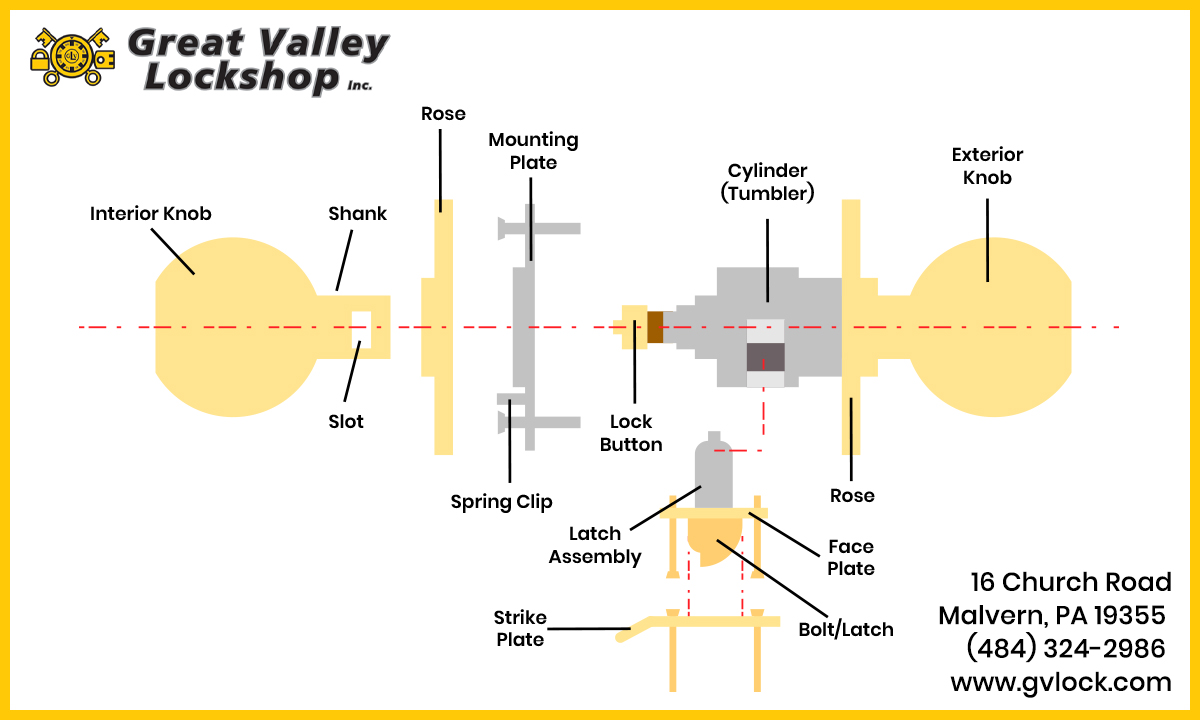
\includegraphics[scale=1.2]{Cylinder-Lock-Diagram.jpeg}
    \caption{Diagram showing the inside of a door lock}
    \caption*{\textit{source: gvlock.com}}
    \label{fig:doorLock}
\end{figure}

\acrlong{covid-19} is the most dangerous infectious disease in the last three years. From the first case in Wuhan City, China, it is a severe pandemic throughout the world. Max Roser, Hannah Ritchie, Esteban Ortiz-Ospina, and Joe Hasell\cite{owidcoronavirus} indicate that from late 2019, there are 176 million confirmed cases, with 3.81 million deaths. In Vietnam, as we experienced in the \acrshort{sars} epidemic in 2003, the situation here is in control now. However, since the pandemic is still a big problem outside Vietnam, according to Havard Health Publishing\cite{harvard_health_publishing_2021}, we should clean frequently touched objects and surfaces regularly and wash our hands often with soap and water. An early stage of prevention is essential in order not to have another outbreak here.

% face recognition
On the other hand, face recognition will solve the problem. As we do not have to touch any surface to verify that we are granted to open the lock, just a simple step is to look at the camera. The hard part is for the local server with a deep learning model to compare the face with a local database.

\begin{figure}[H]
    \centering
    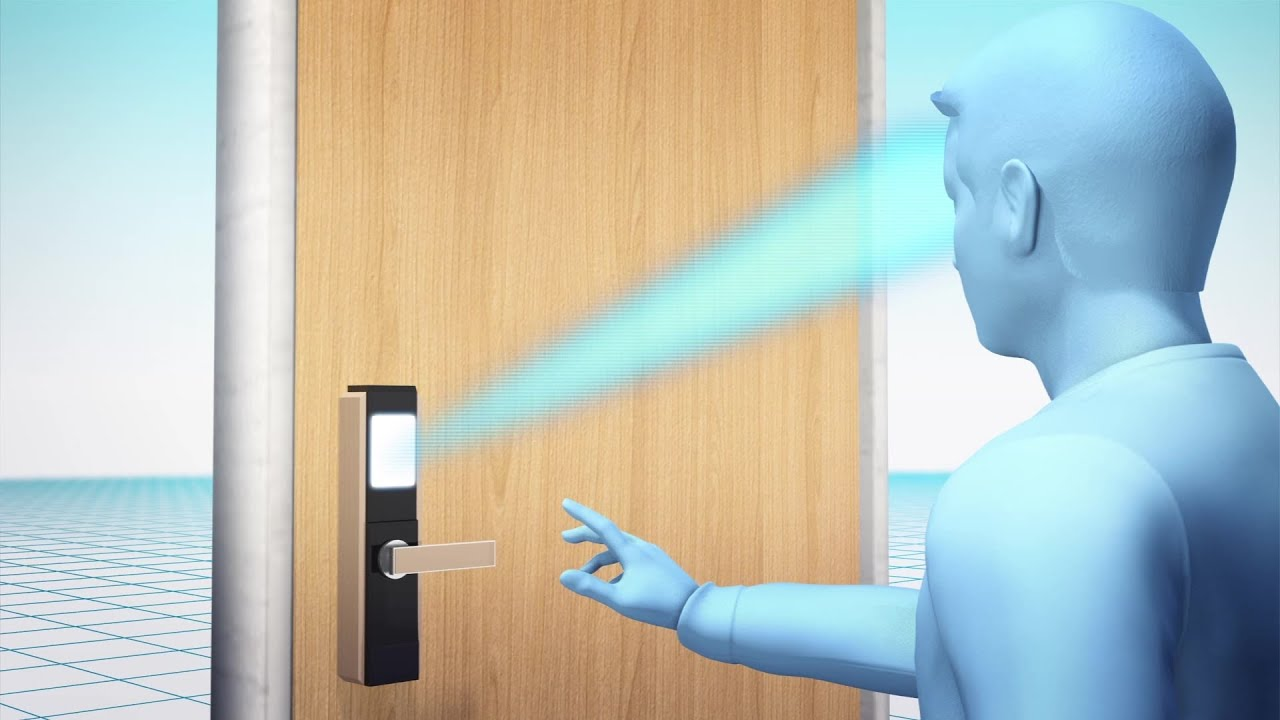
\includegraphics[scale=0.29]{faceRecognitionDemo.png}
    \caption{Door lock integrated with face recognition}
    \label{fig:faceregDoorLock}
\end{figure}

As usual, many researchers in face recognition objects choose to train a model with a large of images for each class. This consumes much time, power to train, and we must re-train the model from scratch if a new person comes. Meanwhile, following to Florian Schroff et al.\cite{DBLP:journals/corr/SchroffKP15} choosing to follow the one-shot learning method can decrease the training model time, which benefits a scale-up in the future. 
\clearpage
\section{Objectives}
\paragraph{}
The main topic of this internship is to improve the accuracy of the deep learning model to classify Asian faces better based on the pre-trained weights on the LFW dataset. It also applies IoT devices for hand-less control for domestic usage and integrates with attendance checks for household and industrial usage. Our goal after the internship is to study and use \acrshort{iot} connectivity, combined with a deep learning model to create a product that uses face recognition to validate if the person is granted to open the door and control smart home devices so that they can do it without hand touch.

The main objectives of this internship include:

\begin{itemize}
    \item Study knowledge of \acrlong{cnn} and implement it on a pre-trained FaceNet\cite{DBLP:journals/corr/SchroffKP15} model.
    \item Propose to apply the Asian dataset to the face recognition model for better performance on recognizing Vietnamese.
    \item Study knowledge of IoT connectivity
\end{itemize}

\section{Thesis Organization}
This report is organized as follows:
\begin{enumerate}
	\item Materials and Methods: presents our dataset, proposed methodology, and the evaluation scenario.
	\item Result and Discussion: presents the evaluation results and discusses our results.
	\item Conclusion and Future-work: conclude the work and presents future research directions.
\end{enumerate}





% ----------------------- CHAPITRE ---------------------------

% \chapter{State of the art}



This chapter must discuss about the different papers addressing the same topics of your internship.
You must be able to explain the work published, by giving the context of the work, the main idea, the main results, and you must also be able to analyze the proposal.

\vspace*{2cm}



You must cite the articles you have read. The citations must be done as follow. \\



\vspace*{2cm}

In the paper \cite{Abr98}, the authors explain how ....

\vspace*{1cm}


The work presented in  \cite{Hau03b} considers the problem of ...


\vspace*{1cm}

In \cite{Ham95}, the results show that .....


\vspace*{1cm}

In comparison with \cite{Hau03a}, the method is ...



% ----------------------- CHAPITRE ---------------------------

\chapter{Materials and Methods}
\label{Materials and Methods}
\paragraph{}

The product contains two main things that need to understand: making the model that is reliable enough to minimize the percentage of allowing a person that is not in the database can control the lock and making the connection between the recognition system to the \acrshort{ccu} fastest, without delay, and most secure. Face recognition plays a role as an authentication layer, allow the action will be authenticated before start. To understand face recognition, we have to study image classification and feature extraction. \acrshort{iot} connection is responsible as a bridge layer to smart devices. Making it fast and instantly is easy, but we have to research blockchain connections for securing the connection.

With the proposed problem, we have split it into more minorissues:

\begin{itemize}
    \item How can we detect faces in the camera stream.
    \item How to capture one frame containing a face from the camera stream.
    \item How to resize the captured frame from a full HD resolution to a smaller size.
    \item How can we verify the face in the captured frame.
    \item Which architecture of the model we are aiming to build.
    \item Which way to connect and control \acrshort{iot} devices.
    \item How to secure the connection between the recognition system to \acrlong{ccu}.
\end{itemize}

To solving above problem, there are some tools and libraries we need to solve it:

\begin{itemize}
    \item \textbf{OpenCV}: Using to resize the original frame to a smaller size, converting the image to grayscale for quickly detecting faces and further reducing the computational complexity. Besides, we need OpenCV to capture frames from a connected camera.
    \item \textbf{Haar Cascade}: Using for detecting faces.
    \item \textbf{\acrlong{mtcnn}}: Help us to extract keypoints of faces. With keypoints, we can measure if the presented face is a real face.
    \item \textbf{One-shot learning}: One-shot learning is used for reducing the retraining model from scratch problem when there is a newcomer.
\end{itemize}

To connect between the face recognition server to \acrlong{ccu} for approving access to control \acrshort{iot} devices, we are using \textbf{Flask} because of its simplicity in development and maintenance.

\section{Materials}

\subsection{OpenCV}
\paragraph{}

\begin{figure}[H]
    \centering
    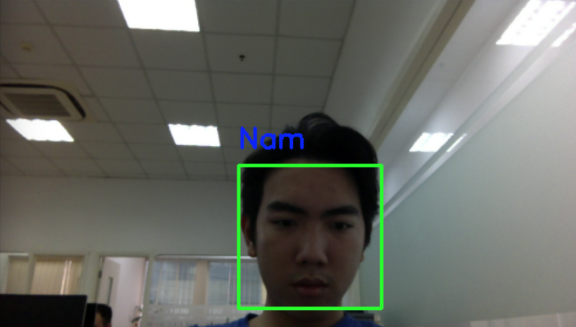
\includegraphics[scale=0.6]{opencvExmaple.png}
    \caption{OpenCV Example}
\end{figure}

OpenCV was introduced at Intel in the year 1999 by Gary Bradsky. The first release came in late 2000. OpenCV represents for Open Source Computer Vision Library. Even though it is written in optimized C/C++, it has interfaces for Python and Java alongside C++. OpenCV has an active user base worldwide, and the number of users is increasing day by day due to the rise in computer vision applications.

OpenCV uses for image and video analysis, like facial detection, license plate reading, photo editing, advanced robotic vision, optical character recognition, and many more. OpenCV-Python is the Python API for OpenCV. It acts like a python wrapper around the C++ implementation of OpenCV.

OpenCV-Python is fast, and it is not difficult to code and deploy(due to the Python wrapper in the foreground). This makes it a great choice to perform computationally intensive programs. 

\subsection{Haar Cascade}
\paragraph{}
The main aim of face recognition is to detect faces in the frame. Haar cascade is one of the fast, effective ways to achieve it. First published by Paul Viola and Michael Jones\cite{haarcascade} in 2001, it is a machine learning approach to detect almost any object, but it mainly solves face detection problems. 

\begin{figure}[H]
    \centering
    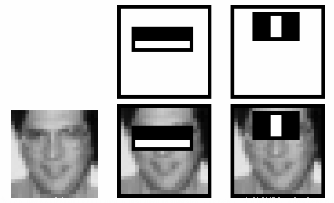
\includegraphics[scale=1.3]{haar.png}
    \caption{Haar Cascades}
    \caption*{\textit{source: docs.opencv.org}}
\end{figure}

Haar Cascade can understand using many \textbf{Haar} features and then using those features many times (\textbf{Cascade}) to build up a face detection. It has four steps: 
Haar Cascade can understand using many \textbf{Haar} features and then using those features many times (\textbf{Cascade}) to build up to face detection. It has four steps: 

\subsubsection{Haar Feature extraction}

\begin{figure}[H]
    \centering
    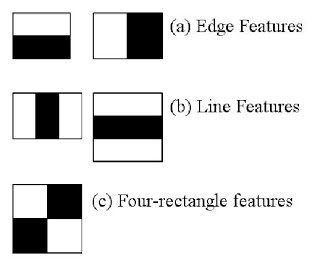
\includegraphics[scale=0.7]{haar_features.png}
    \caption{Four Haar Features}
    \caption*{\textit{source: docs.opencv.org}}
    \label{fig:haarFeature}
\end{figure}

First, we have to collect the Haar feature. As a feature to encode every domain is operate faster than pixel system, objects are mainly classified on many simple features. A \textbf{Haar Feature} is a calculation performed on adjacent rectangular regions on a specific location in the window. Haar Feature is shown in figure~\ref{fig:haarFeature} below.

\subsubsection{Integral Image Representation}
Integral Images efficiency speed up the calculation of these Haar features in one pass over the image. It creates sub-rectangles and creates array references for each sub-rectangles instead of computing at every pixel—figure~\ref{fig:integralImage} followed by Zhang, Cha, and Zhang, Zhengyou \cite{book}.

\begin{figure}[H]
    \centering
    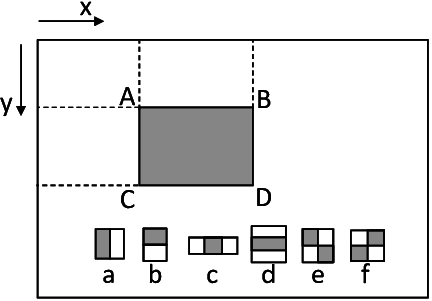
\includegraphics[scale=0.6]{integralImage.png}
    \caption{How integral image works}
    \label{fig:integralImage}
\end{figure}

\subsubsection{Adaboost Training}
As we do not know which Haar classifier is the best fit, we have a solution to group every weak classifier into a robust classifier using \textbf{Adaboost} (adaptive boosting). It chooses the best features and trains the classifier to use them. 

\begin{figure}[H]
    \centering
    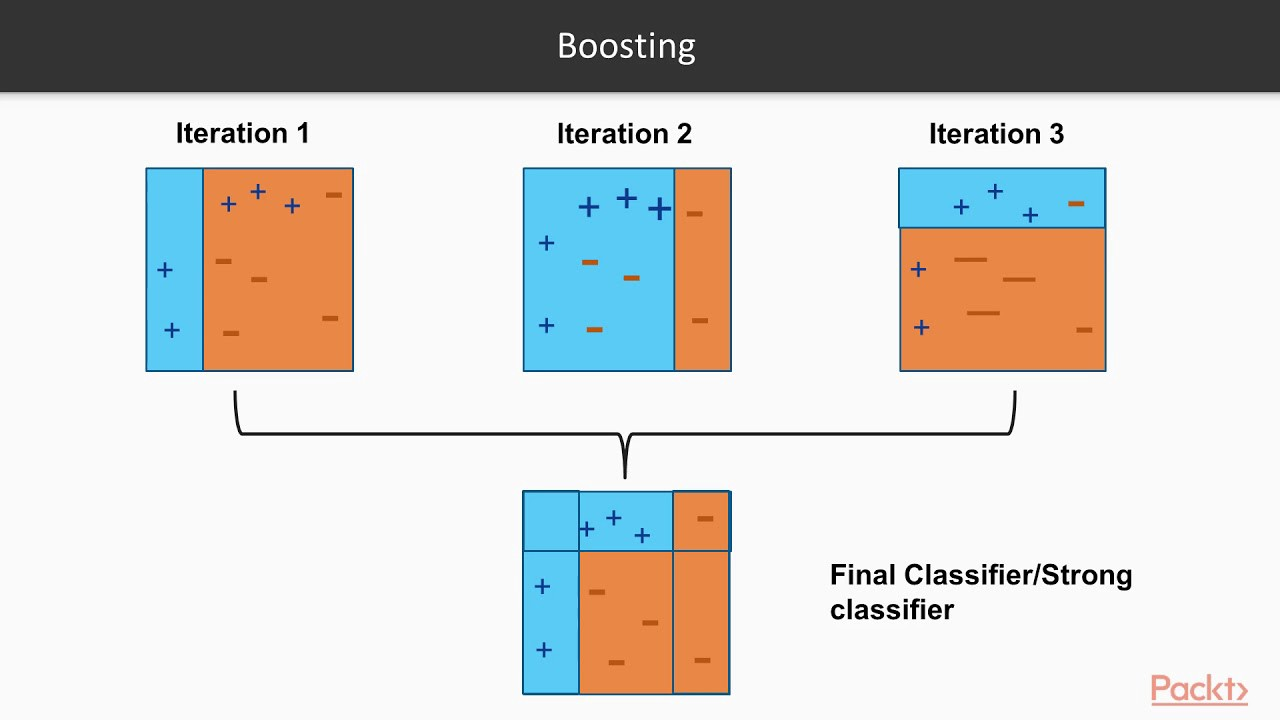
\includegraphics[scale=0.2]{adaptiveBoost.png}
    \caption{Adaptive boosting algorithm}
    \caption*{\textit{source: Packt}}
\end{figure}

\subsubsection{Cascading Classifier Architecture}
Paul Viola and Michael Jones ensured in their paper that employing a \textbf{cascade of classifiers} makes the algorithm performs faster. The cascade classifier consists of series of stages, and each stage contains a collection of strong classifiers. It removes the need to apply all features on a window simultaneously. Every time the sub-window slides into a window, if it detects the face, we move to the next step; else, we discard that region and slide to another part. The rejected region will keep at rejected sub-windows. The process is shown in diagram\ref{fig:cascadeStructure}, originally from Lee, Deok Gyu et al.\cite{article}.

\begin{figure}[H]
    \centering
    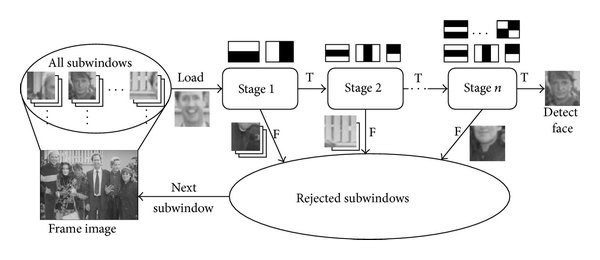
\includegraphics[scale=0.8]{cascadeStructure.jpeg}
    \caption{Cascade structure of Haar classifier}
    \label{fig:cascadeStructure}
\end{figure}

\subsection{\acrlong{mtcnn}}
\paragraph{}
\acrlong{mtcnn} (\acrshort{mtcnn}) is a solution for both face detection and face alignment. Proposed by Zhang et al.\cite{Zhang_2016}, it is one of the most popular and accurate face detection tools today. This model has three \acrlong{cnn} (P-Net, R-Net, O-Net) connected in a cascade.

\begin{figure}[H]
    \centering
    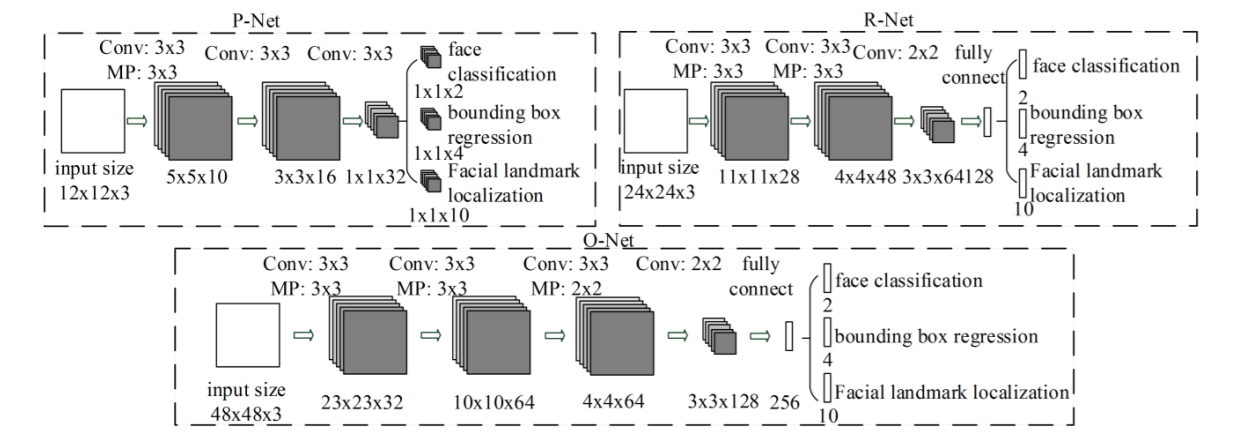
\includegraphics[scale=0.4]{mtcnnArchitecture.png}
    \caption{MTCNN structure}
\end{figure}

\acrshort{mtcnn} can integrate both recognition and alignment because of multi-task learning. There are three-stage corresponding to three \acrshort{cnn}. In the first stage, the Proposal Network (P-Net) quickly produces windows thanks to a shallow \acrshort{cnn}. The Refine Network (R-Net) refines the proposed candidate windows into a more complex \acrshort{cnn} to the second stage. Lastly, Output Network (O-Net) is more complicated than others, refining the result and showing the facial landmark positions.

\subsection{One-shot learning}
\label{oneShot}
\paragraph{}
One-shot learning is a supervised algorithm that only needs one or only a few pictures for each class. We use a simple \acrshort{cnn} algorithm to predict who it is from the input picture of one class.

\begin{figure}[H]
    \centering
    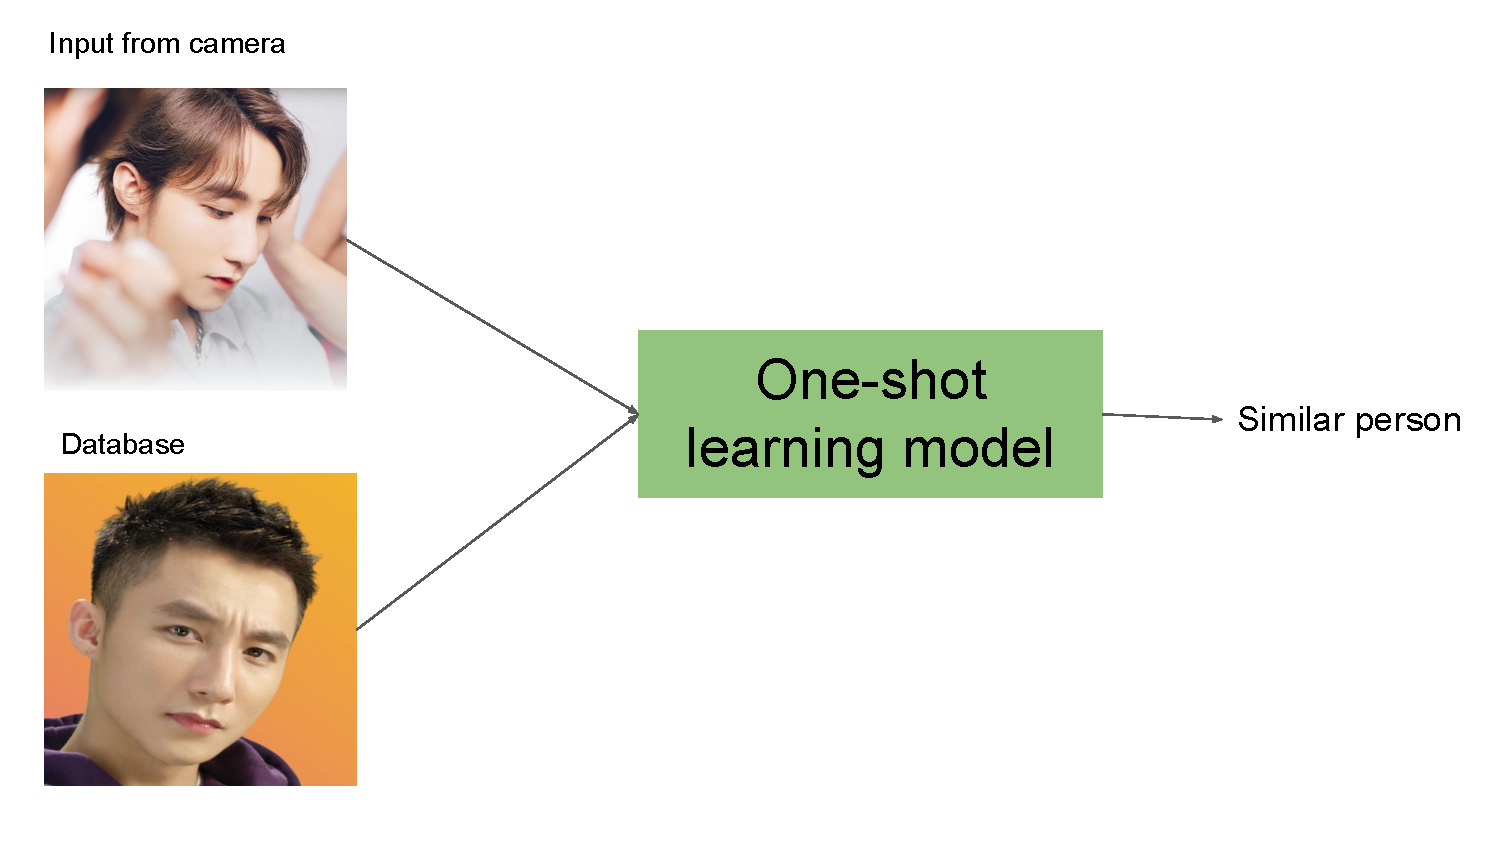
\includegraphics[scale=0.5]{oneShotLearning.pdf}
    \caption{One-shot learning example}
\end{figure}

This method will save much man’s power and power consumption. Because we only a little picture, every time newcomers show up, we will make it easier by taking only one picture of them. And the process of creating embeddings for existing images is also taking less time than the traditional way that is training a model with thousands of pictures for each class. We can scale up the system for a large number of classes quickly.

\subsection{Learning similarity}
\paragraph{}
Learning similarity is based on a distance calculation between two pictures, usually a $\ell_1$, $\ell_2$ norm so that if that is the same person, the distance will be smallest, else it will be biggest:

\begin{center}
    $
    \begin{cases}
    d(img1,img2) \leq \tau \Rightarrow \text{same}\\
    d(img1,img2) \geq \tau \Rightarrow \text{different}\\
    \end{cases}
    $
\end{center}

When using this method, we have to choose a threshold to decide if this picture is the same or different. For example, in figure~\ref{fig:learnSimilar}, if the image from the left has a distance smaller than the threshold, which is 0.2, then it is the same picture:

\begin{figure}[H]
    \centering
    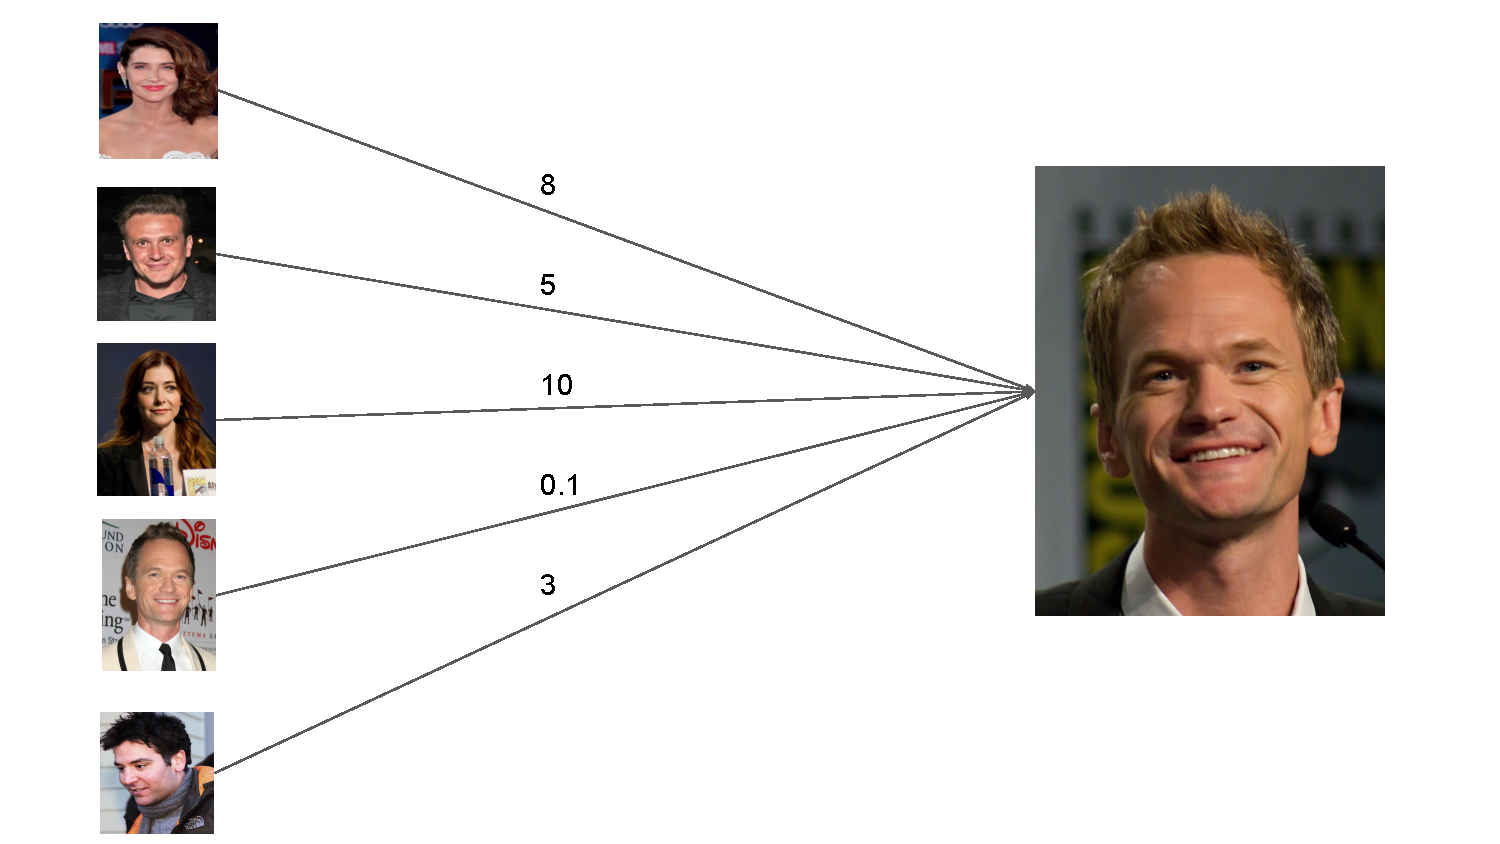
\includegraphics[scale=0.5]{learningSimilarity.pdf}
    \caption{Learning similarity method}
    \label{fig:learnSimilar}
\end{figure}

We can see that learning similarity has the advantage that we can find the similarity picture without re-training the model again. Besides, it will not depend on the number of classes. So we do not have to train the model again when there is a new class. 

\subsection{Siamese neural network}
\label{sec:siamese}
\paragraph{}
Siamese network was first introduced by Yaniv Taigman et al.\cite{inproceedings}. It is a network architecture that can answer if two pictures are the same person in it. The architecture of a Siamese network is a \acrlong{cnn} without an \textbf{output layer} to encoding a picture to an embedding vector. The input of a Siamese network is two random pictures chosen from the database. After the network handling it, it returns two vectors corresponding to two input pictures. The \textbf{loss function} is responsible for calculating the distance between two vectors to show the difference between them. Usually, the loss function in this network is a $\ell^2$-norm function.

\begin{figure}[H]
    \centering
    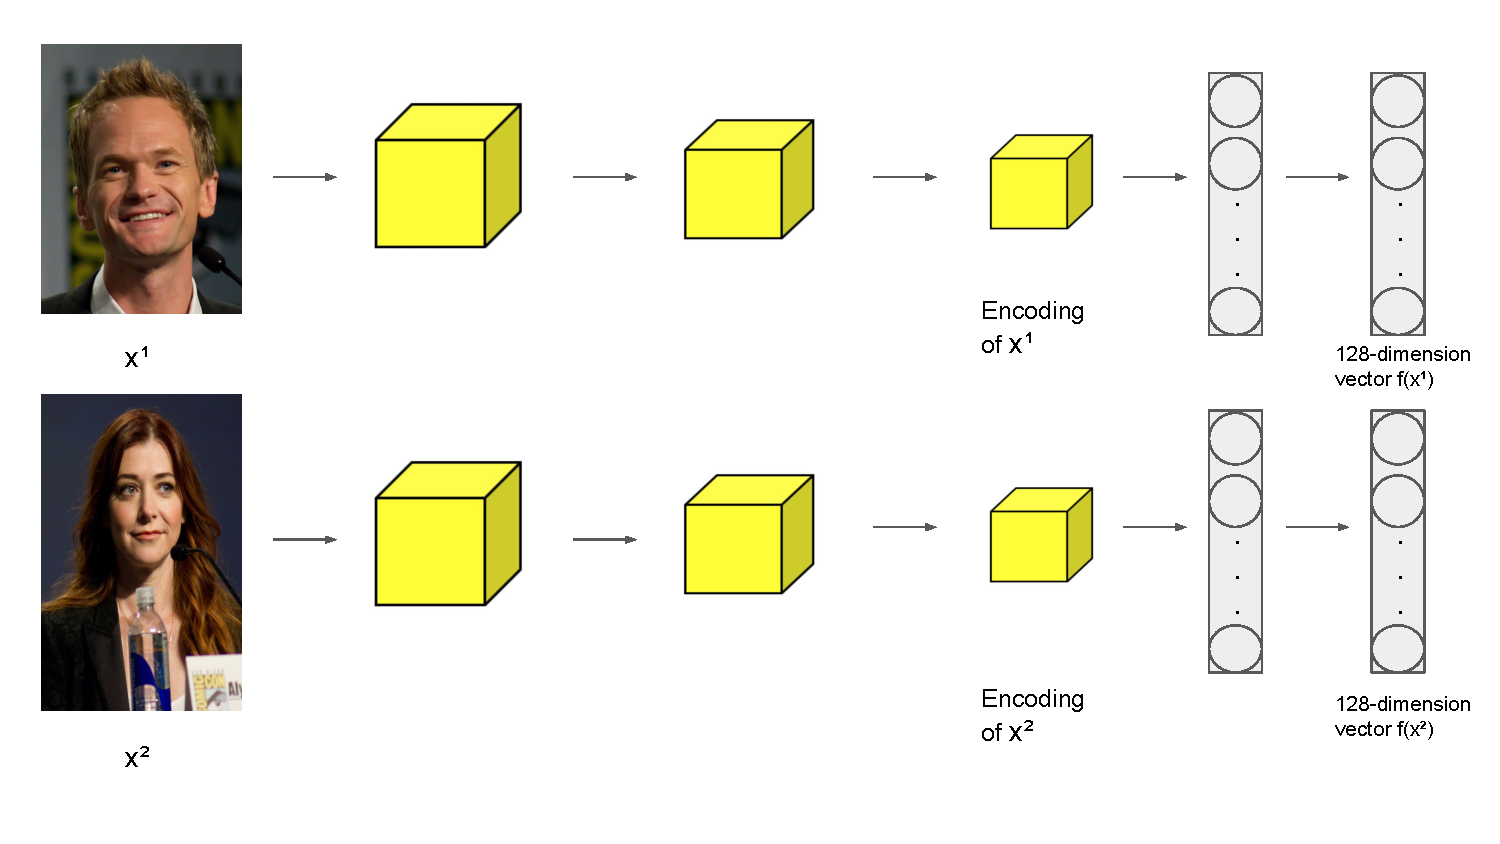
\includegraphics[scale=0.5]{siameseNetwork.pdf}
    \caption{Example of Siamese network}
    \label{fig:siameseNet}
\end{figure}

We conclude if two pictures were the same person by this function:

\begin{center}
    $
    \delta(x_1,x_2) = 
    \begin{cases}
        min ||f(x_1)- f(x_2)|| & \text{two person are the same} \\
        max ||f(x_1)- f(x_2)|| & \text{two person are different} \\
    \end{cases}
    $
\end{center}

\subsection{\acrlong{cnn}}
\paragraph{}

\acrfull{cnn} is a Deep Learning neural network that can take structured arrays of data like images, analyzing properties, aspects from the input images to differentiate one from the other. The name \acrlong{cnn} shows that it employs the mathematical convolution operation. We can stack up layers inside it for our purpose. For example: with three layers, the network can recognize handwriting; with 25 layers, the network can recognize human faces. We can add more layers for extracting and recognizing more features.

\begin{figure}[H]
    \centering
    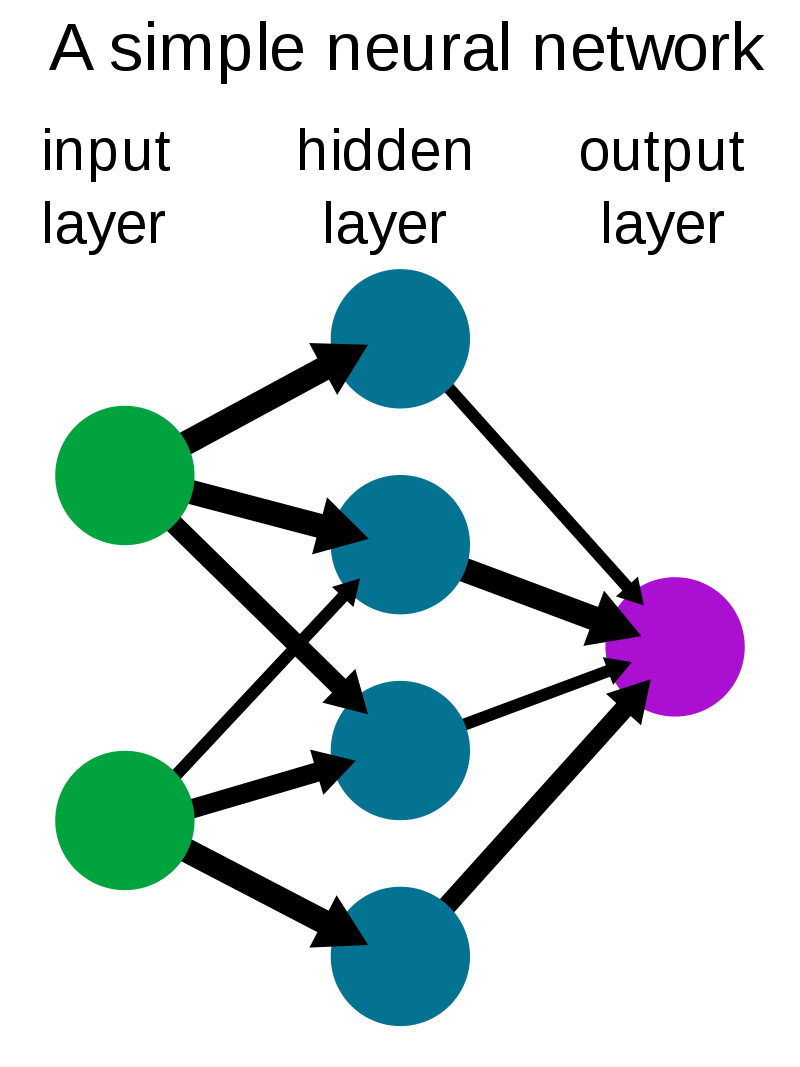
\includegraphics[width=0.3\textwidth]{Neural_network.png}
    \caption{Simple neural network}
    \caption*{\textit{source: Wikipedia}}
    \label{fig:simpleCNN}
\end{figure}

The \acrshort{cnn} was typically built by three main layers:

\begin{itemize}
    \item \textbf{Input layer}: takes input images then fits them into the network.
    \item \textbf{Hidden layers}: contains layers that perform a specific task.
    \item \textbf{Output layer}: decide which one belongs to which class.
\end{itemize}

We can control how many layers are inside hidden layers, but there are three main layers in it:
\begin{itemize}
    \item {Convolutional layer}: This layer extracts features from the image by taking the dot product between the image and a set of a learnable parameter known as the kernel. The kernel is smaller than the image but more in depth. 
    
    \begin{figure}[H]
        \centering
        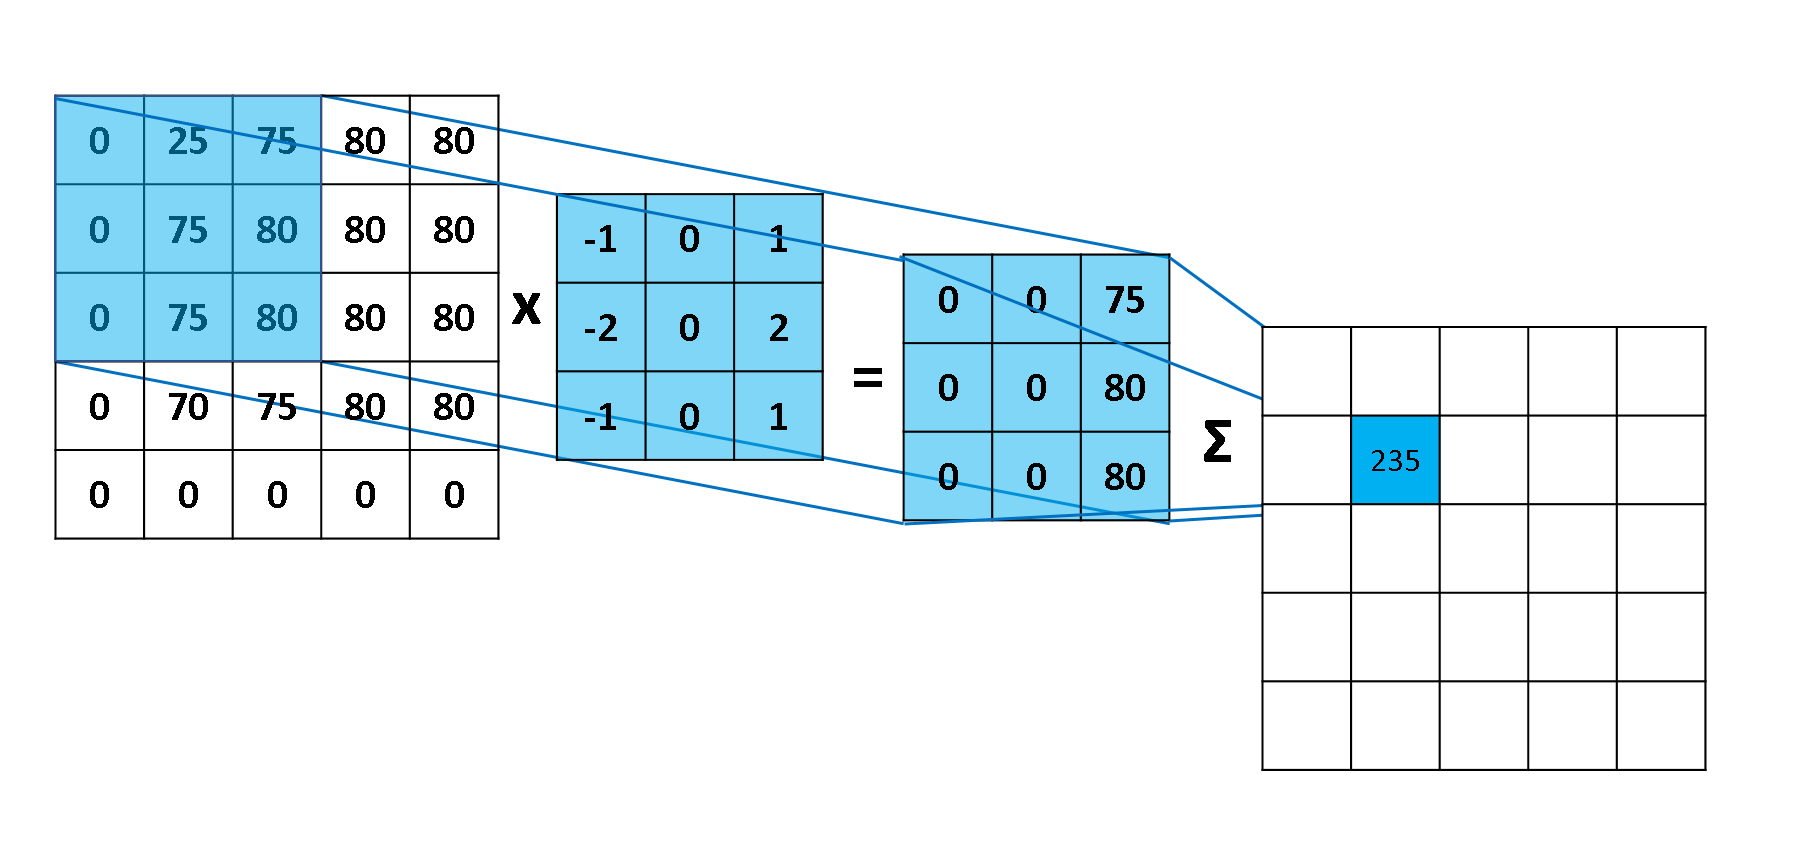
\includegraphics[width=0.7\textwidth]{convolutional_layer.png}
        \caption{Convolutional layer}
    \end{figure}
    During the forward pass, the kernel slides across the image, creating a two-dimensional image representation. The sliding size of the kernel is called \textbf{stride}. The bigger stride, the faster the kernel slide across the image.
    
    It can be seen that the feature map should be smaller if the kernel size is bigger. To avoid reducing feature map size after every convolutional layer, we have \textbf{padding} with value zero for having the image and feature map in the same size. The model contains many feature maps for extracting features from the input. It includes a stack of feature maps with different kernel values to extract clear features.
    
    \item {Activation layer}: The Activation layer is put at the end or between the \acrlong{cnn}. It helps to calculate the argument for the next layer. We have different activation functions like Rectified Linear Unit (ReLU), sigmoid, and softmax. Commonly ReLU is used after the Convolutional layer, sigmoid and softmax are used at the classification output layer.
    
    \begin{figure}[H]
        \centering
        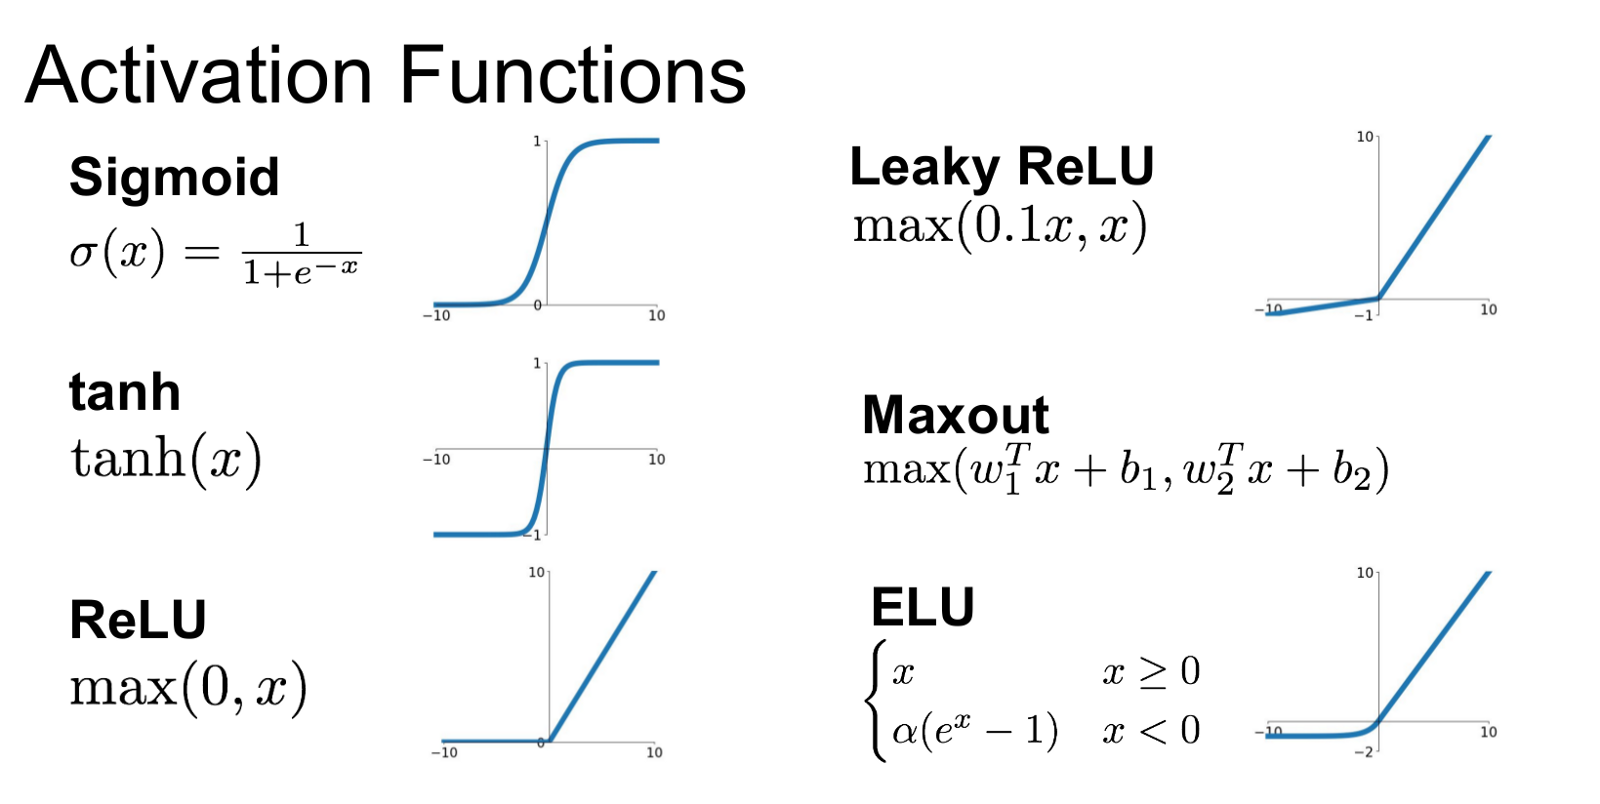
\includegraphics[scale=0.3]{activationLayer.png}
        \caption{Activation functions}
    \end{figure}
    
    \item {Pooling layer}: The pooling layer replaces the output of the network at some locations by deriving summary statistics of nearby outputs. It reduces the number of parameters and computations in the network, spatial size of the network to control overfitting. 
    
    There are two operations in this layer:
    
    \begin{itemize}
        \item Max Pooing: like its name states, it takes the max value from a pool.
        \begin{figure}[H]
            \centering
            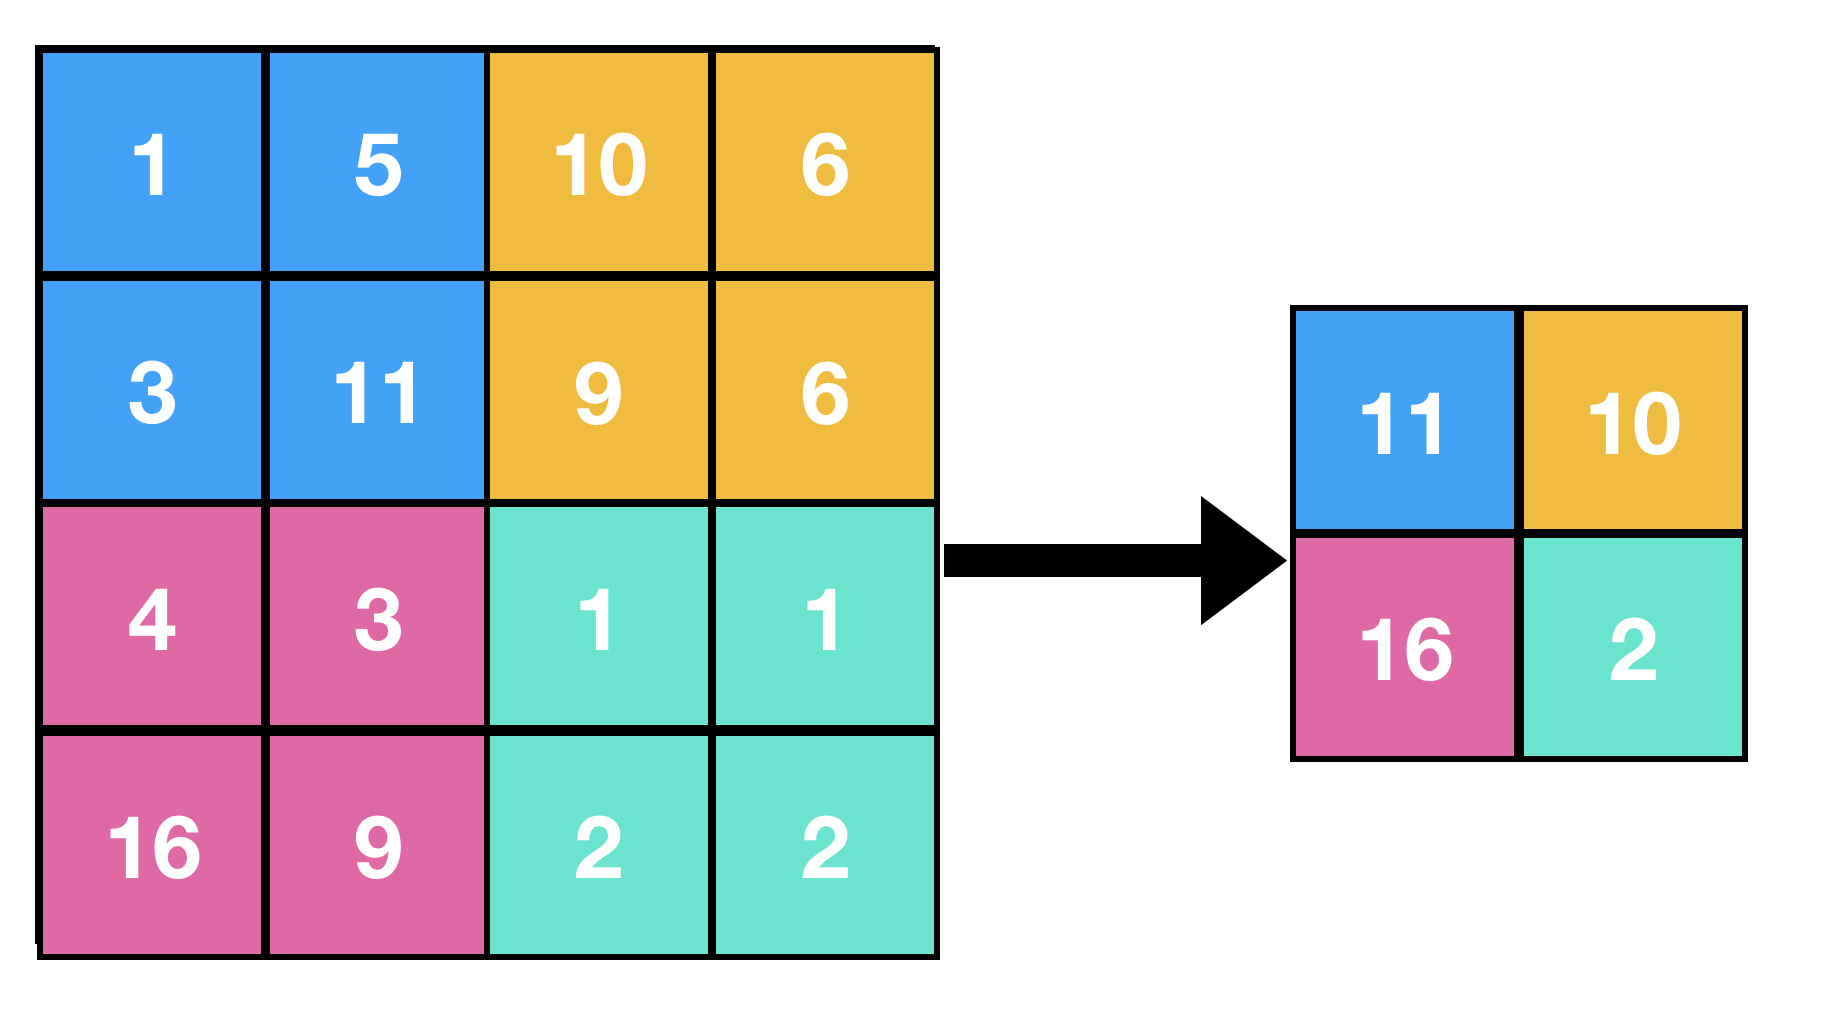
\includegraphics[width=0.3\textwidth]{Maxpooling.png}
        \end{figure}
        
        \item Average Pooing: it takes the average values from all value from a pool.
        \begin{figure}[H]
            \centering
            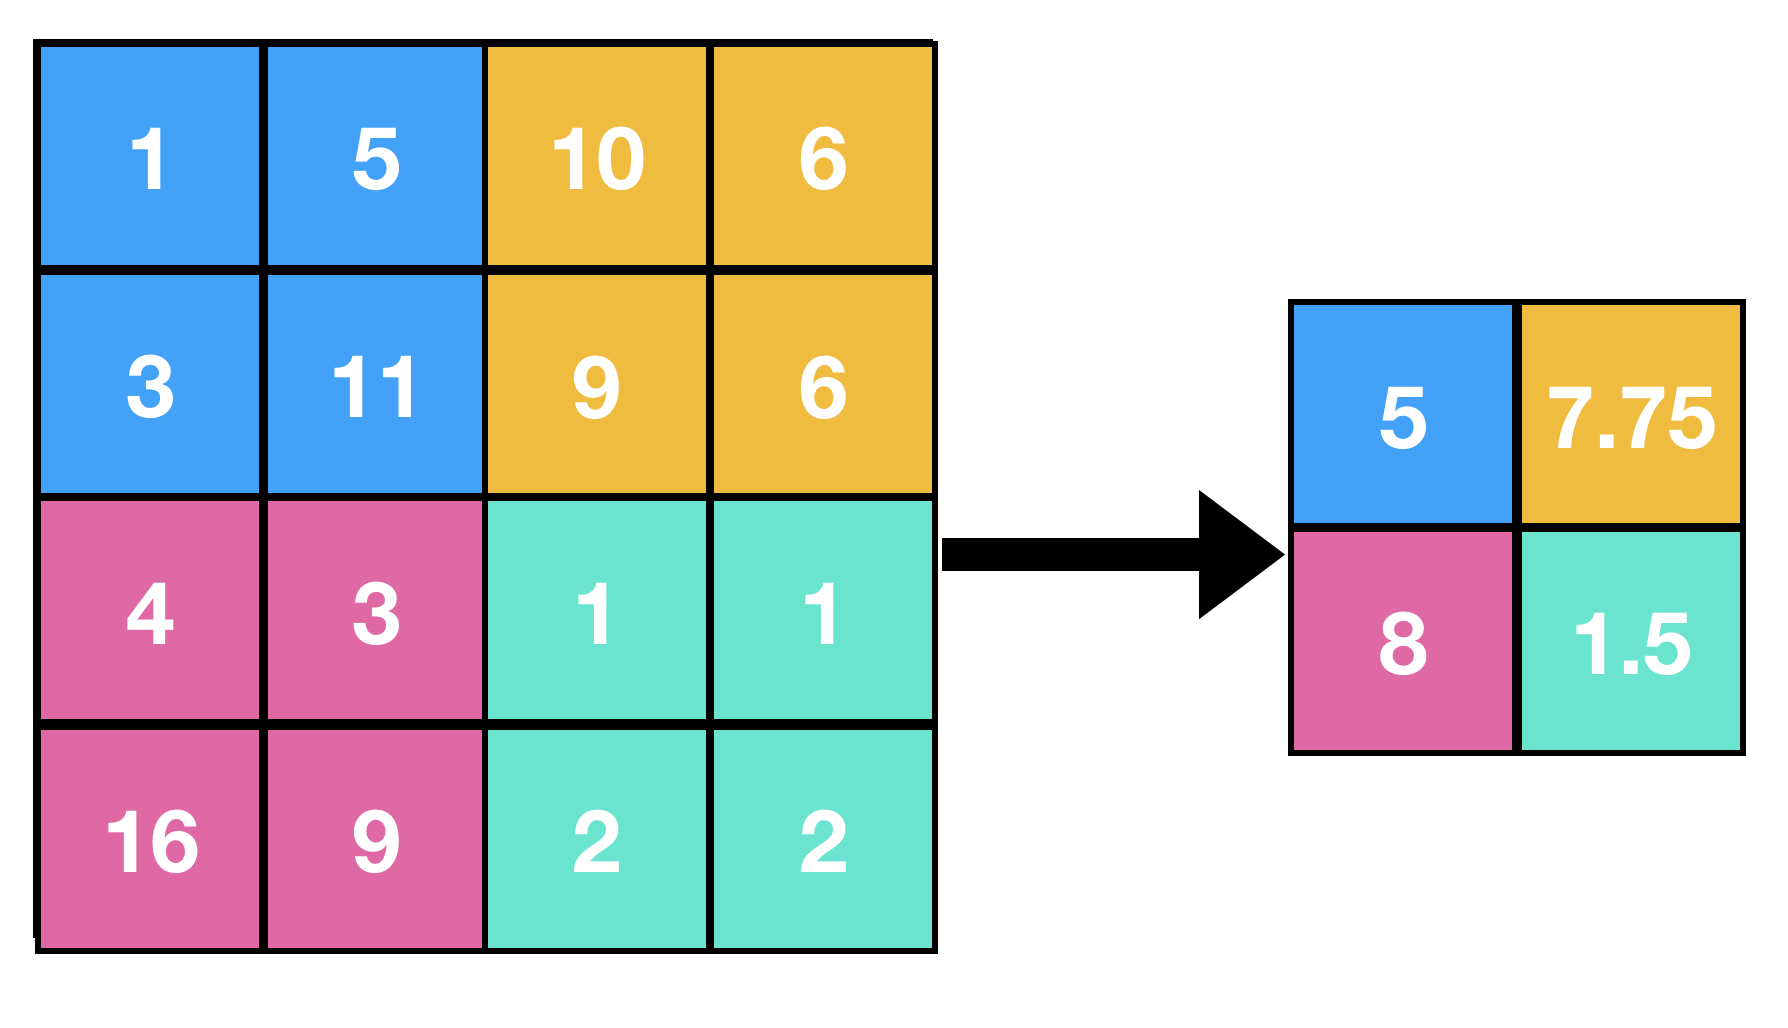
\includegraphics[width=0.3\textwidth]{Avgpooling.png}
        \end{figure}
    \end{itemize}
    
    \item {Fully Connected layer}: Neurons in this layer have a complete connection with all neurons from the previous layers. It can be computed by matrix multiplication followed by a bias offset. Fully Connected layers compile data extracted from earlier layers to get the final output.

    \item {Dropout layer}: Randomly drop connection from the previous layer.
    
    \item {Batch Normalization}: Normalize and scale data after each activation.
    
\end{itemize}

The combination of all these above layers is the basic concept of the \acrshort{cnn} model, as in figure \ref{fig:cnnDesign}.

\begin{figure}[H]
    \centering
    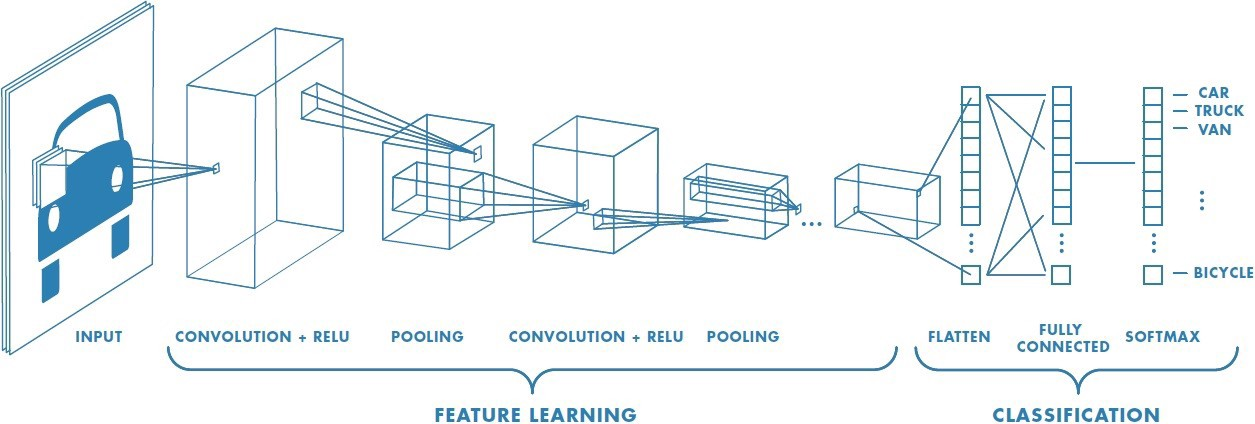
\includegraphics[scale=0.3]{convolutionalNetwork.jpeg}
    \caption{Basic concept of \acrshort{cnn}.}
    \label{fig:cnnDesign}
\end{figure}

\subsection{Flask}
\paragraph{}
Flask is a micro web framework written in Python. Flask takes advantage of the simplicity of Python, which makes it easy to build a primary application to backend APIs. It is classified as a micro-framework because it does not require any libraries. 

It is also called a \acrlong{wsgi} (\acrshort{wsgi}) framework. Flask gives us many choices when developing web applications and provides the necessary tools to build and deploy a web. Here are some of the merits of using Flask: 

\begin{enumerate}
    \item \textbf{Easy to use}: Flask framework is easy to understand. The simplicity in the framework helps us to navigate around and create applications easily.
    \item \textbf{Very flexible}: Most of the components of Flask can be altered. It allows users to customize the website.
    \item \textbf{Testing}: It allows unit testing through its integrated support, built-in development server, fast debugger, and RESTful request dispatching.
\end{enumerate}

\clearpage
\section{Methods}

\subsection{Building a Face recognition system}

\subsubsection{FaceNet}
\paragraph{}
In 2015, Florian Schroff et al.\cite{DBLP:journals/corr/SchroffKP15} introduced FaceNet. It transforms the face image into 128 dimensions Euclidean space, similar to word embedding. Once the FaceNet model having been trained with triplet loss for different classes of faces to capture the similarities and differences between them, the 128-dimensional embedding returned by the FaceNet model can be used to clusters faces effectively. It is the backbone of many open-source face recognition models like OpenFace\footnote{\url{https://cmusatyalab.github.io/openface/}}, facenet\footnote{\url{https://github.com/davidsandberg/facenet}}, etc.

\begin{figure}[H]
    \centering
    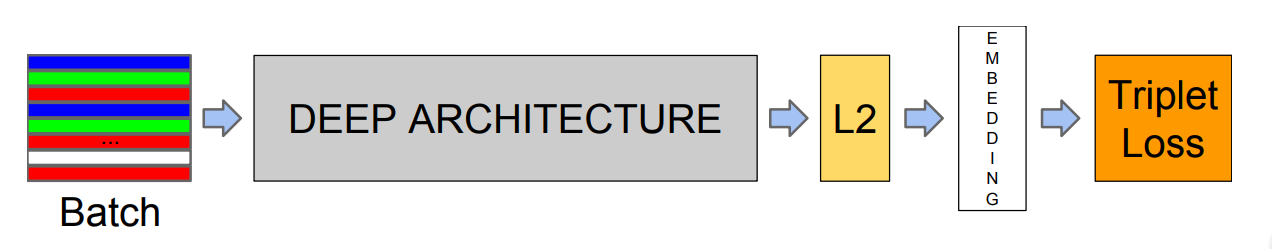
\includegraphics[scale=0.5]{facenetArchitecture.png}
    \caption{FaceNet Architecture}
\end{figure}

FaceNet has solved two problems in face recognition algorithm before it:
\begin{enumerate}
    \item Apply a \acrshort{cnn} and use 128-dimensional data to not need a bottleneck layer for reducing data dimensionally.
    \item Loss function can learn the similarity between two pictures in the same class or distinguish two pictures in different classes simultaneously.
\end{enumerate}

This model outputs an embedding of image $f(x)$ with $L_2$ normalization on it. After that, these embeddings pass into a loss function to make the squared distance between two images is small when two images belong to the same identity, whereas the squared distance will be significant. This loss function is called \textbf{Triplet loss}. 

\subsubsection{Triplet loss}
\label{tripletLoss}
\paragraph{}
The encoding of the \acrlong{cnn} helps us encode the picture into a 128 dimensional vector $f(x)$ called embedding. It is normalized such that:

\begin{center}
    $||f(x)||^2_2=1$
\end{center}

To implement Triplet loss, we need to take three pictures, including: anchor picture ($x^a_i$), positive picture ($x^p_i$) which is a picture of the same person), negative picture ($x^n_i$) which is from the different person, to satisfy that:

\begin{center}
    $||f(x^a_i) - f(x^p_i)||^2_2 + \alpha < ||f(x^a_i) - f(x^n_i)||^2_2$
\end{center}

$\alpha$ is an enforced margin to differentiate between positive and negative pairs. So that the loss function can be defined:

\begin{center}
    $\mathcal{L}(x^a,x^p,x^n)=\Sigma^n_i[|f(x^a_i) - f(x^p_i)||^2_2 - ||f(x^a_i) - f(x^n_i)||^2_2 + \alpha]$
\end{center}

\begin{figure}[H]
    \centering
    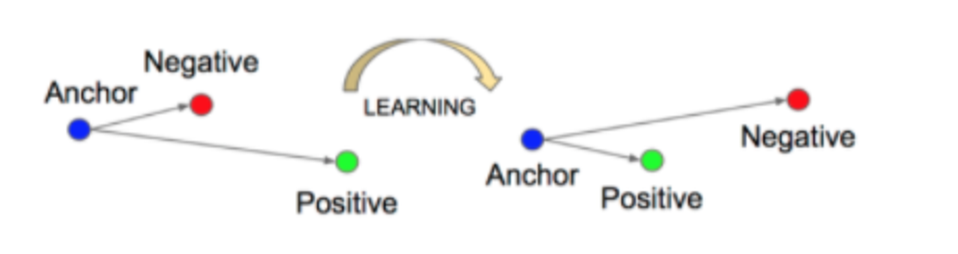
\includegraphics[scale=0.5]{tripletLoss.pdf}
    \caption{Triplet loss learning}
\end{figure}

If the above function can easily be satisfied by choosing close triplets, it would not help the training. So choosing triplets that violate that function is essential.

\subsubsection{Triplet images input selection}
\paragraph{}
If the chosen triplets were easy to distinguish, the learning images would not make any sense. We need to choose hard triplets to make the model harder to learn and help the model discriminate effectively between faces.

\begin{figure}
    \centering
    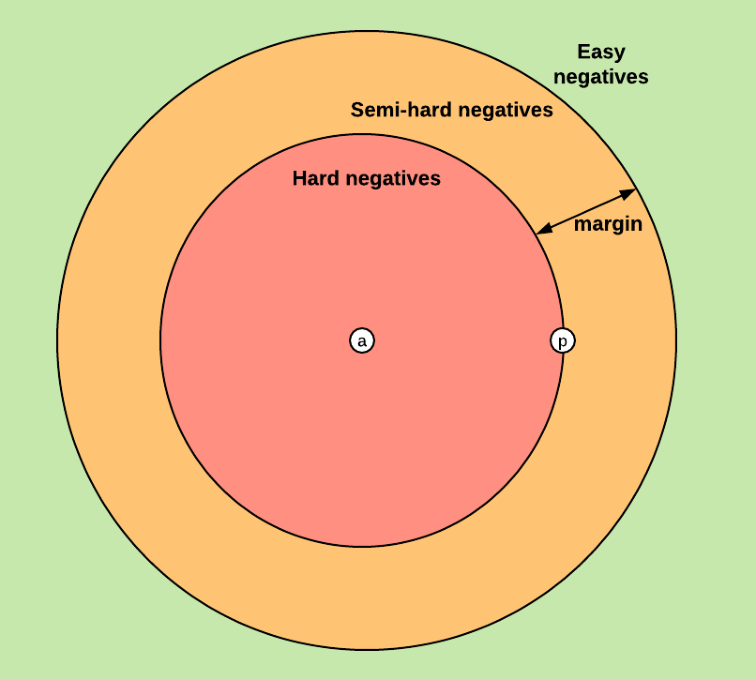
\includegraphics[scale=0.5]{tripletSelection.pdf}
    \caption{Chossing hard triplets}
\end{figure}

This mean that for a given $x^a_i$, we need to choose 2 pairs of anchor-positive and anchor-negative to please:
\begin{enumerate}
    \item Hard positive: $\argmax(|f(x^a_i) - f(x^p_i)||^2_2)$
    \item Hard negative: $\argmin(||f(x^a_i) - f(x^n_i)||^2_2)$
\end{enumerate}

Computing \textbf{Hard positive} and \textbf{Hard negative} can do on the previous checkpoint or do it on every mini-batch to minimize computationally expense when generating the whole training data set. Choosing triplets on purpose can make the model giving the result more accurate. 

\subsubsection{Experimental with pre-trained FaceNet model}
\paragraph{}
Based on \hyperref[sec:siamese]{Siamese neural network}, we will choose a based network and drop out the output layer. VGG16 is one of the most powerful networks in the classification topic. It contains multi-layers of Convolutional, Pooling, and Fully Connected layers. The input runs through two convolutional layers with 64 filter channels of 3*3 kernel with the same padding from the input. Following a Max Pool layer of stride 2*2, two layers have convolution layers of 256 filter channels with filter size 3*3. Then there is a Max Pooling layer of stride 2*2, following by two convolution layers of filter size 3*3 and 256 filter channels. There are two sets of 3 convolution layers and a max pool layer, and each has 512 filters of 3*3 sizes with the same padding. After all, the data is passed through three fully connected layers.

\begin{figure}[H]
    \centering
    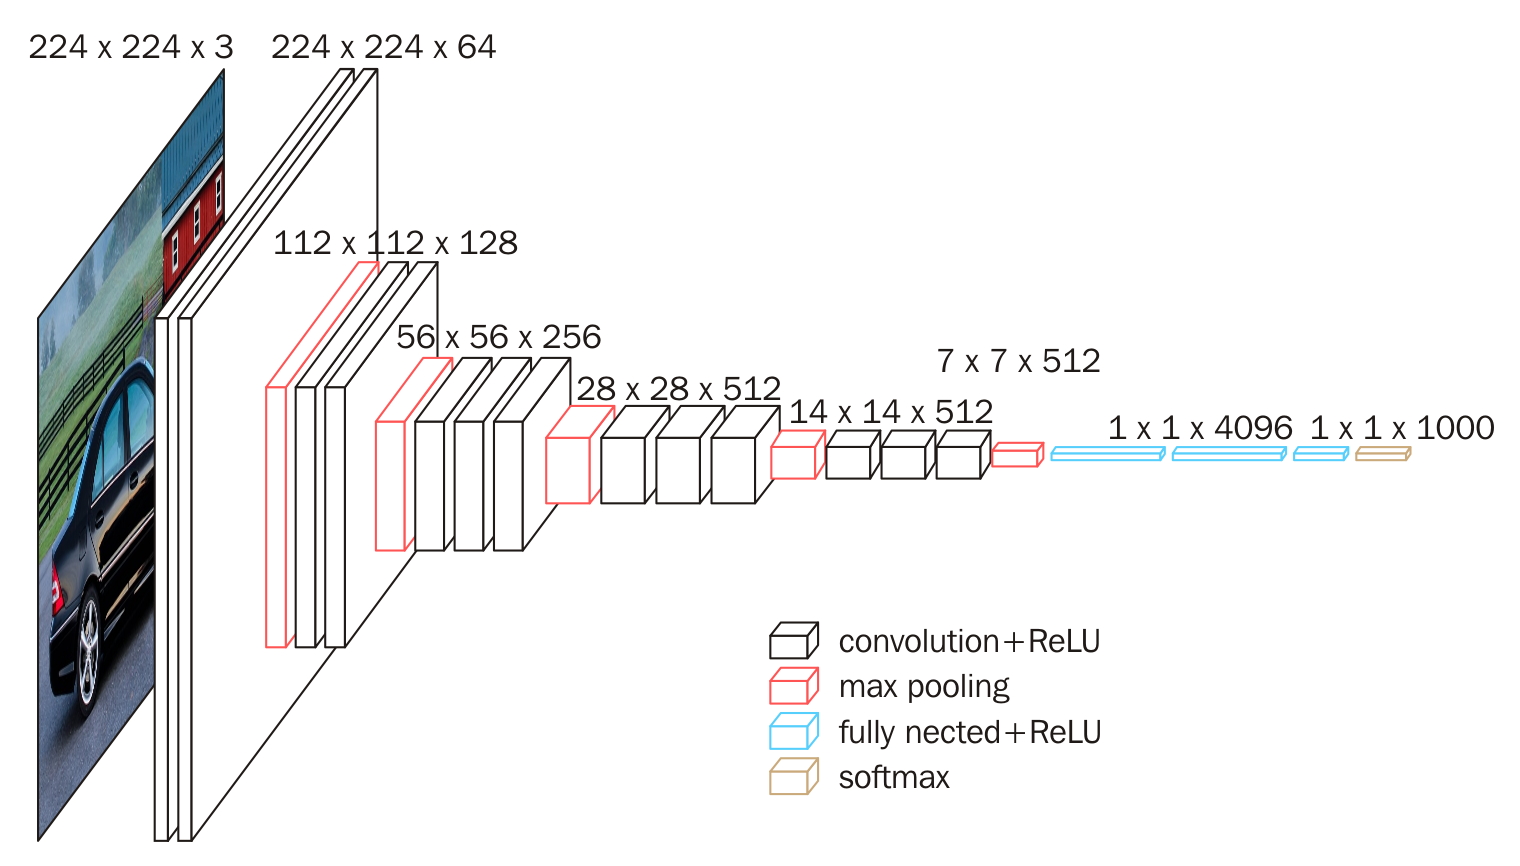
\includegraphics[width=0.8\textwidth]{VGG16.png}
    \caption{Architecture of VGG16 network.}
    \caption*{\textit{source: towardsdatascience.com}}
    \label{fig:VGG16}
\end{figure}

After getting the base network, we add the Triplet loss function to determine the input belongs to which class. To save training time, we are using the weights from OpenFace\footnote{\url{https://cmusatyalab.github.io/openface/}} model. We will train the model with VN-celeb dataset, published by Sun* AI team, to use this with Vietnamese people.

\subsubsection{Making the recognition system}
\paragraph{}
We are using the trained model, OpenCV, and MTCNN to create the system. To avoid using an image to spoof the system, we are setting up two lights from behind the camera. If someone came with a picture, the system would not detect it.

First, we are connecting the camera to the server. The server has a job that captures every frame that contains the human face with the help of OpenCV. The model implemented on the server creates embedding vectors for every registered face in the database. Moreover, these vectors are stored only in the running state and deleted after the system stops to avoid outside access.

After that, the system creates an embedding vector for the current face that shows at the camera, which is detected using Haar Cascade. Compare with a recent detecting model like dlib\footnote{\url{https://github.com/davisking/dlib}}, \acrshort{mtcnn}\cite{Zhang_2016}, OpenCV \acrshort{dnn} Face Detector, Haar Cascade shows some outdated and worst result in detecting faces in a picture that has many faces in that or large picture size. Besides, it also depends much on lighting, face rotation, and the quality of the image. But during the recognition, there is only one person at the camera at that time. And faces in the database with face in the camera are equal in lighting and quality. So using the Haar Cascade is the best option for us at the detecting time.

\begin{figure}[H]
    \centering
    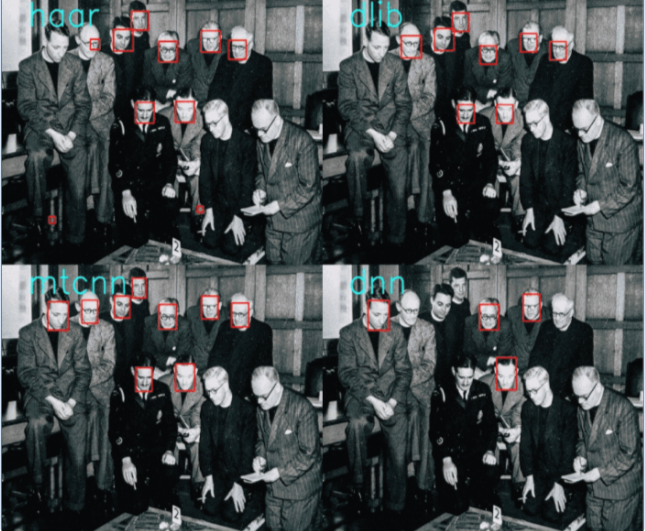
\includegraphics[scale=0.6]{comparisonHaar.png}
    \caption{Comparison along with face detection model}
    \caption*{\textit{source: Vardan Agarwal - towardsdatascience.com}}
\end{figure}

Since we got vectors from the database and the vector from the camera, the system will calculate the Euclidean distance with these vectors to find the smallest compare with the threshold we choose.

After the recognition is finished, the liveness test will continue. The liveness test is for avoiding people using a printed image to trick the system. We are using \acrshort{mtcnn} to extract key points from the face. It will store the default key points of the face. \acrshort{mtcnn} detector will track the key points. When it satisfies the math function of calculating the distance of eyes and nose, the system will request the \acrlong{ccu}.

\begin{figure}[H]
    \centering
    \includegraphics{dataflow.png}
    \caption{Recognition system data flow}
\end{figure}

\subsection{\acrshort{iot} devices setup and API connection}
\subsubsection{\acrshort{iot} devices setup}
\paragraph{}
\acrshort{iot} is one of the buzzwords in the technology industry in the past years, stands for \acrlong{iot}. \acrshort{iot} means all of the things that are connected to the Internet and can be controlled remotely. According to Wikipedia\footnote{\url{https://en.wikipedia.org/wiki/Internet_of_things}}: 
"..the network of physical objects - devices, vehicles, buildings, and other items - embedded with electronics, software, sensors, and network connectivity that enables these objects to collect and exchange data."

The main factor in the upwards trend in \acrshort{iot} systems is DIY (do it yourself) electronic platforms like Raspberry Pi and Arduino. Raspberry Pi (figure~\ref{fig:raspi}) has many advantages: small, inexpensive, easy to use, etc. And after all, it allows us to connect various accessories via a 40-pins \acrshort{gpio} connection built-in on board.

\begin{figure}[H]
    \centering
    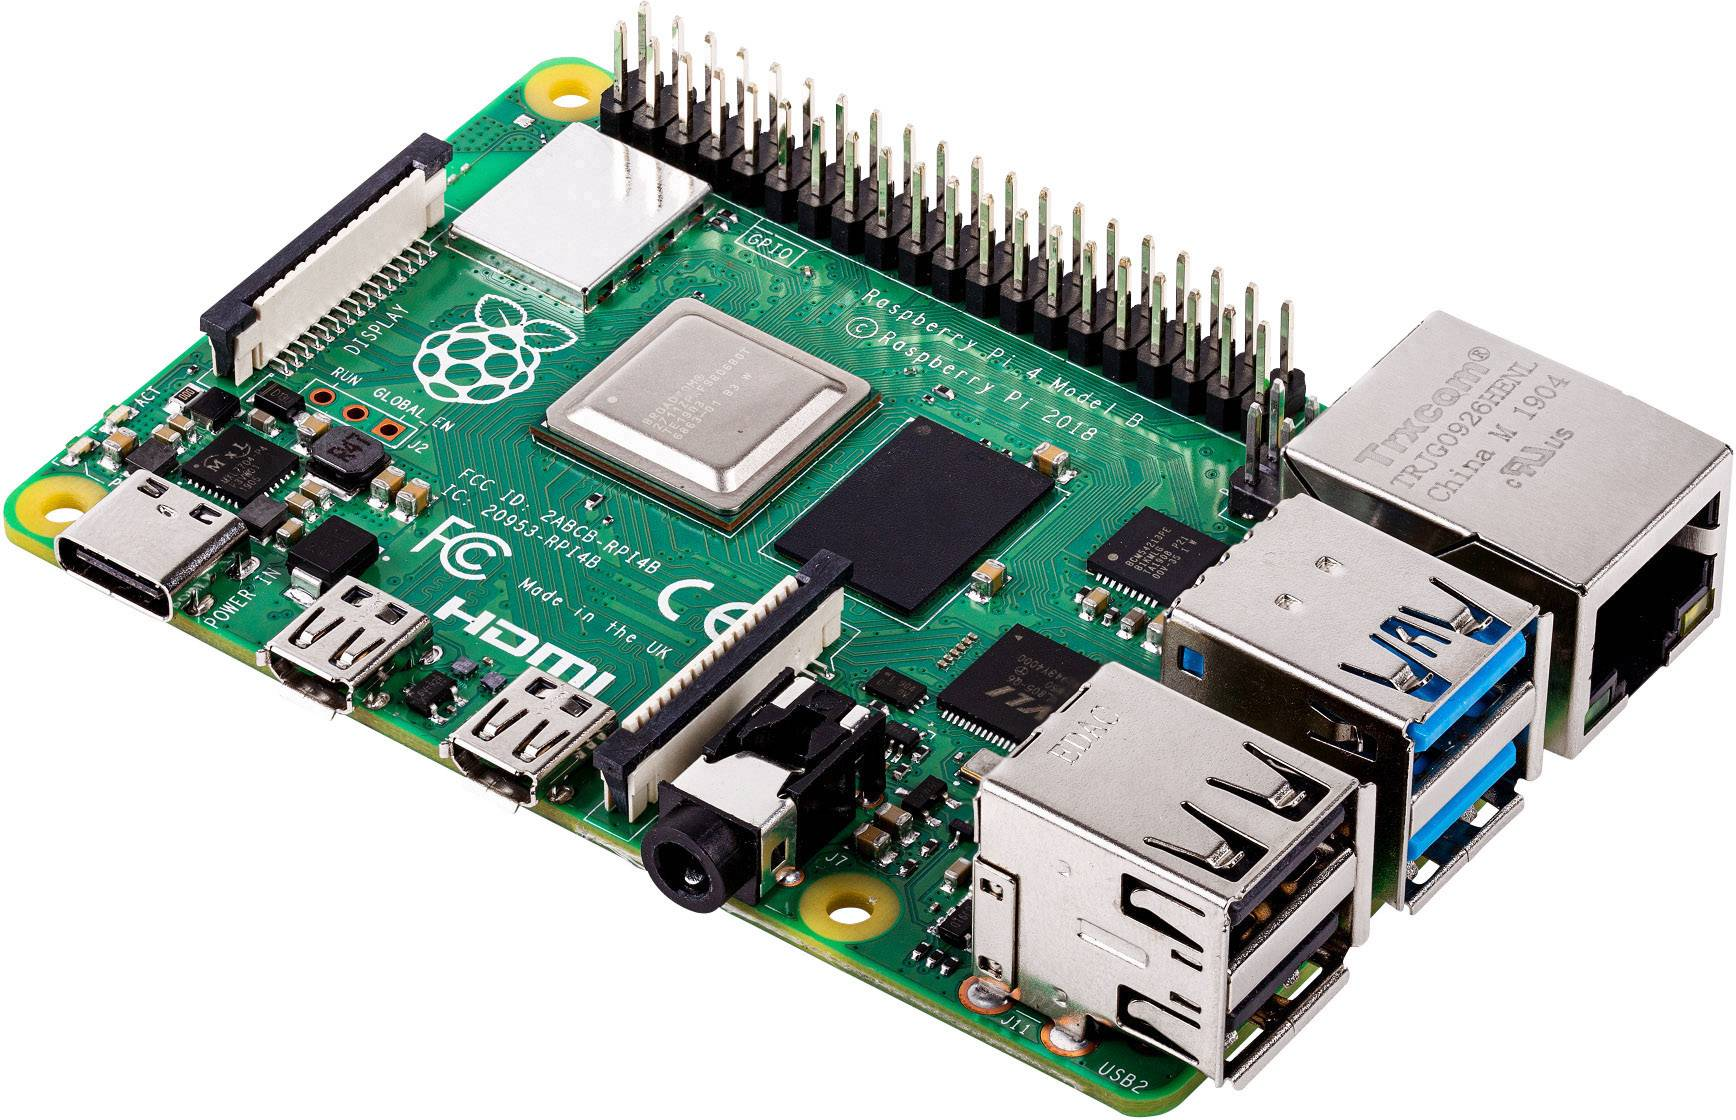
\includegraphics[scale=0.15]{raspPi.png}
    \caption{Raspberry Pi board}
    \label{fig:raspi}
\end{figure}

To interact with all \acrshort{iot} devices, we use Raspberry Pi version 4 with a specification in table~\ref{tab:raspiSpecs} as a \acrshort{ccu}(\acrlong{ccu}).  

\begin{table}[H]
    \centering
    \caption{\acrlong{ccu} specification}
    \begin{tabular}{|c|c|}
        \hline
        OS & Raspberry Pi OS \\
        \hline
        Kernel version & 5.10\\
        \hline
        CPU & Quad-core Cortex-A72 (ARM v8) 64-bit Soc \\
        \hline
        RAM & 4GB\\
        \hline
    \end{tabular}
    \label{tab:raspiSpecs}
\end{table}

Since the limitation of the voltage output of the \acrshort{ccu} device, we are controlling one electric door lock and two light bulbs. The diagram of connecting electric door lock is in figure~\ref{fig:doorLockDiag}

\begin{figure}[H]
    \centering
    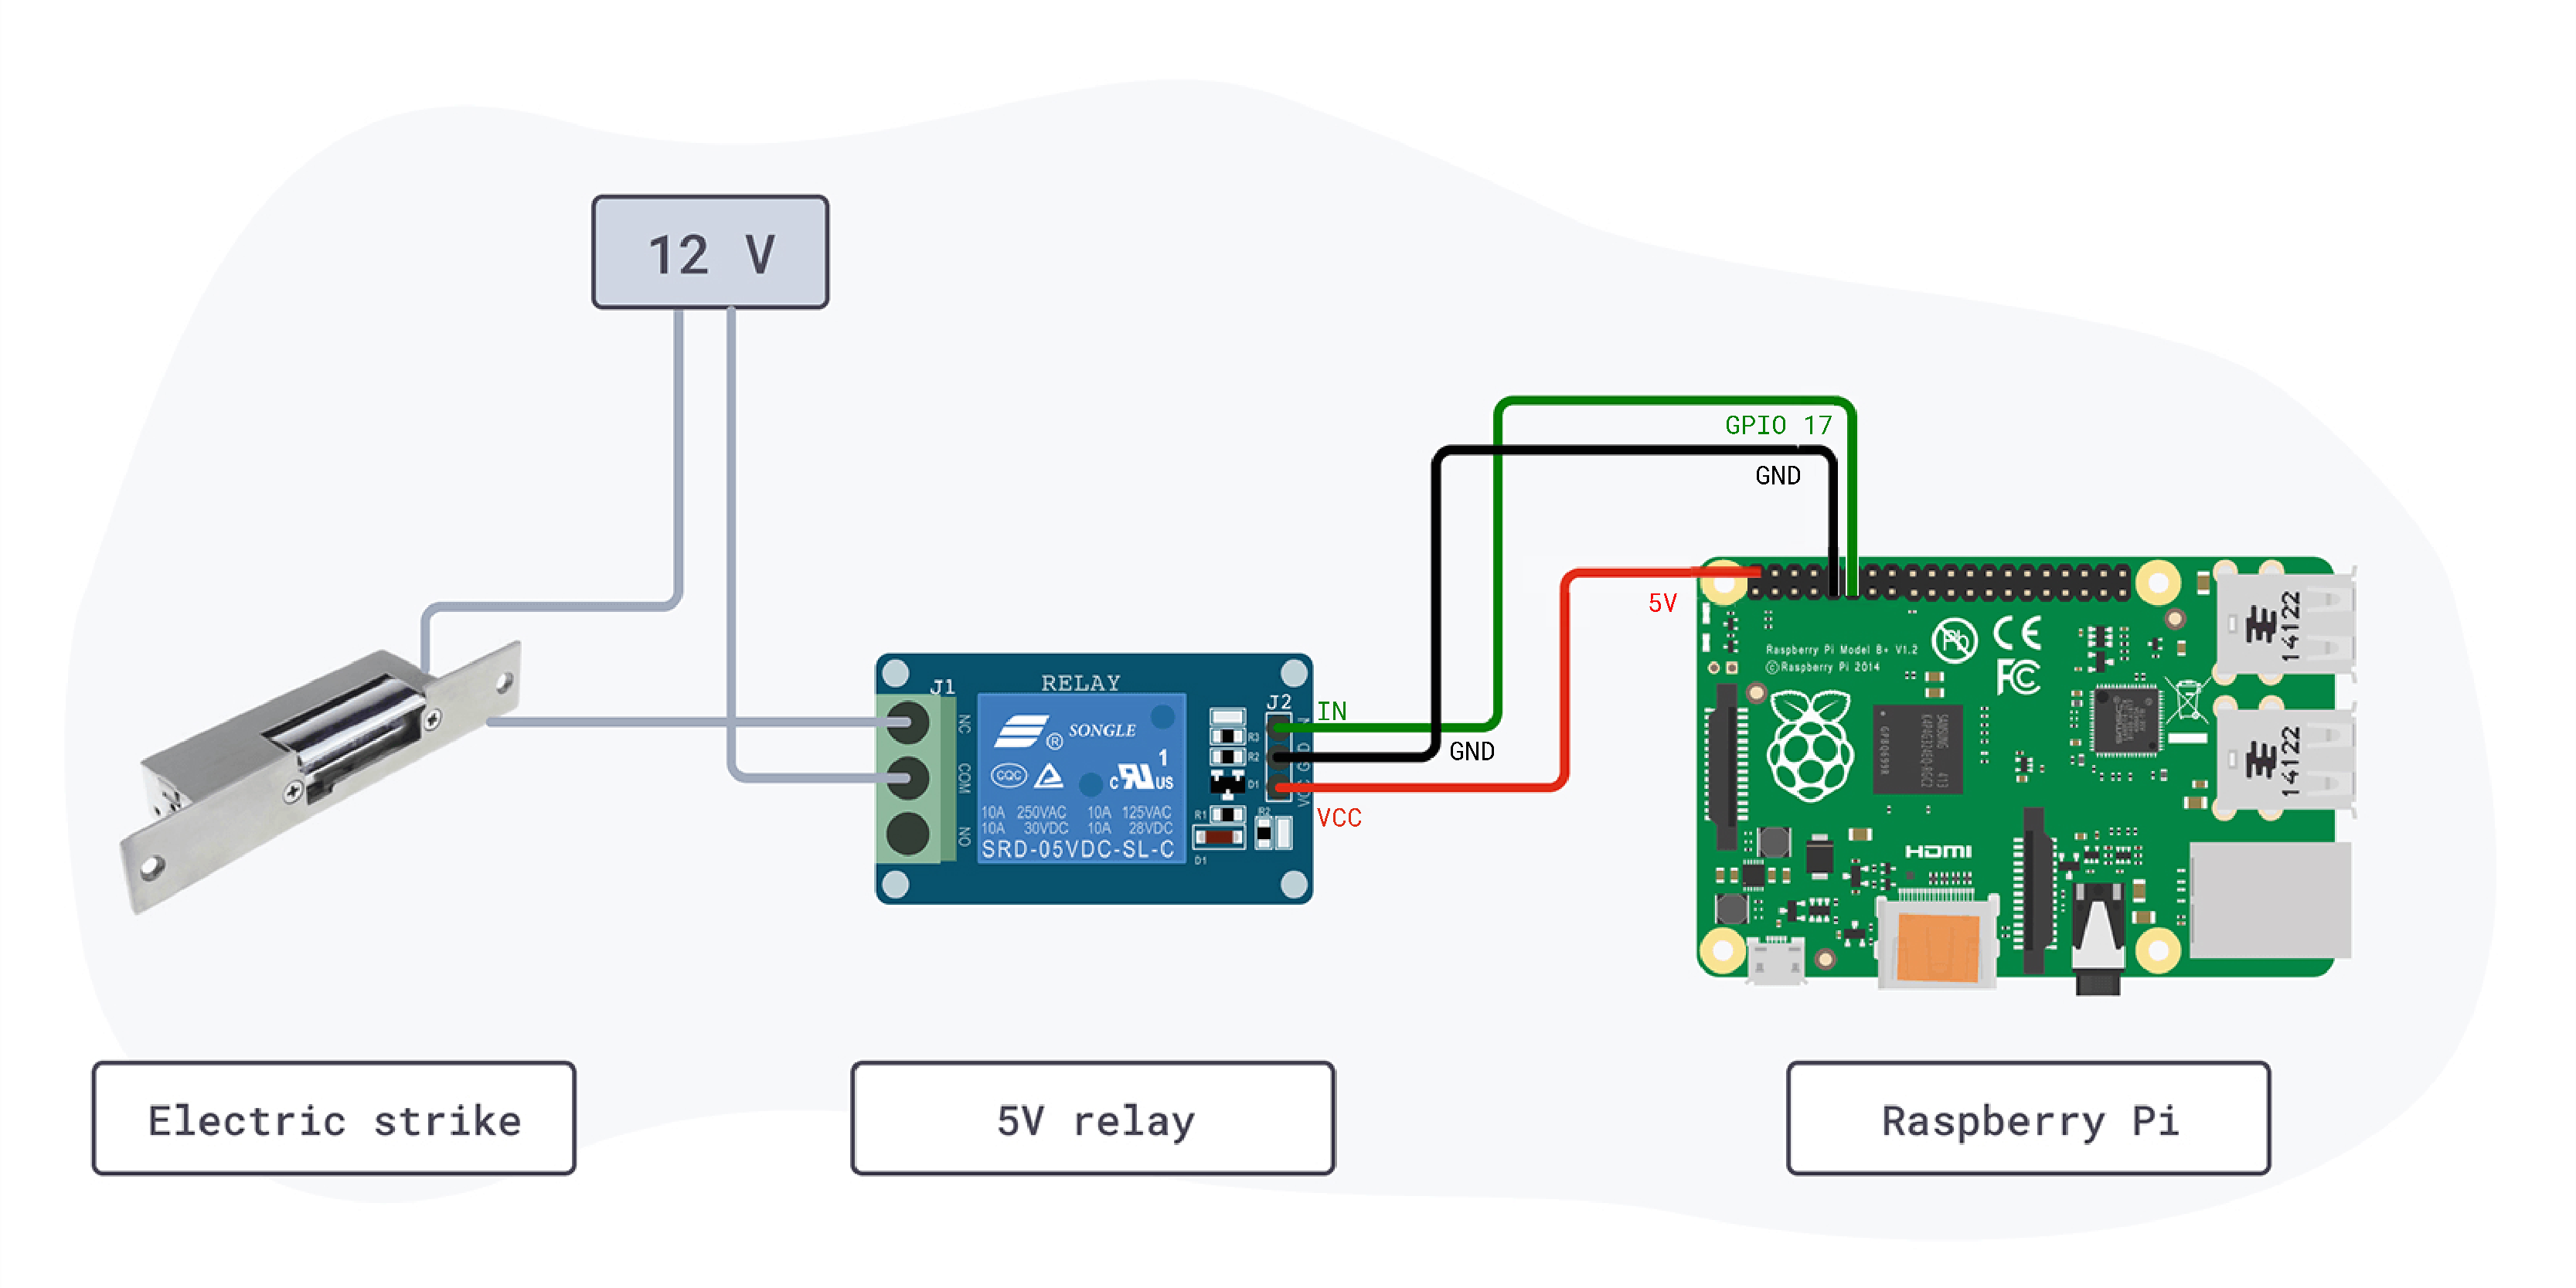
\includegraphics[scale=0.2]{piSetup.pdf}
    \caption{Electric door lock connection diagram}
    \label{fig:doorLockDiag}
\end{figure}

We are using a 12V DC lock. So we connect the lock with a 12V external power, which is three 3.7V 18650 batteries. We are using a 5V relay for controlling the switch with code. The connection between \acrshort{ccu} and relay: connect \textbf{5V \acrshort{gpio} pin} to \textbf{VCC} for power to the relay, \textbf{GND pin} to \textbf{GND} for ground, \textbf{\acrshort{gpio} 17} to \textbf{IN} for controlling.

The central part of controlling the lock is connecting the lock and external power to the relay. Here we connect the lock to \textbf{\acrshort{nc}} (\acrlong{nc}); External power to \textbf{\acrshort{com}} (\acrlong{com}). The \acrshort{com} connection is the moving part of the relay. We set the initial state of the INPUT from \acrshort{ccu} as \textbf{GPIO.low}, High/Low switch on the relay to \textbf{High}. This setup works from the initial setup before; If the input from \acrshort{ccu} is low, then the lock does not have any power equal to lock state; else, if the input is high, then the lock has power equal to unlock state. We are setting the lock state to \textbf{GPIO.low}, unlock state to \textbf{GPIO.high}.

For light bulbs, the setup is much simpler:

\begin{figure}[H]
    \centering
    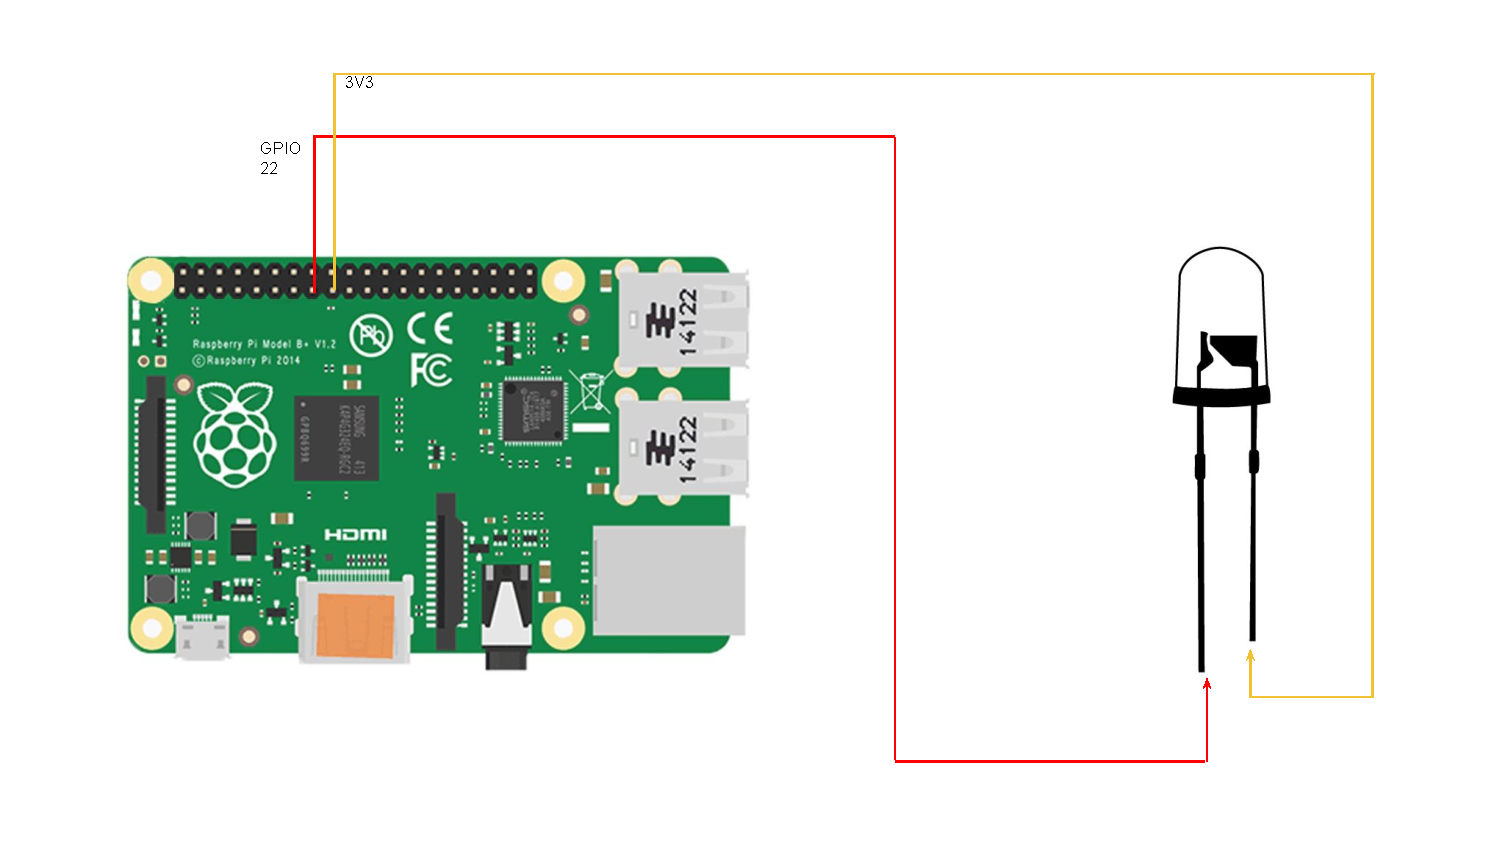
\includegraphics[scale=0.4]{lightSetup.pdf}
    \caption{Light bulbs connection diagram}
\end{figure}

We connect one pin to \textbf{GPIO 22} pin to control, the other to a \textbf{3V3} pin for power. We set automation for every unlock, and the light turns on for two minutes for a home scenario.

\subsubsection{Google Assistant \acrshort{sdk}}
\paragraph{}
The best way to set up a smart home with \acrshort{iot} devices is automation. Because of the limitation of our \acrshort{ccu}, adding Google Assistant \acrshort{sdk} to it will extend the ability to connect more smart devices using the Google Home network.

Google Developers team has clear documentations\footnote{\url{https://developers.google.com/assistant/sdk/guides/service/python#steps}} about how to implement it on a Raspberry Pi using Python.


\subsubsection{\acrshort{api} connection}
\paragraph{}
To connect a server for Face recognition to \acrlong{ccu}, we create an \acrfull{api} using Flask to link these two components.

\begin{figure}[H]
    \centering
    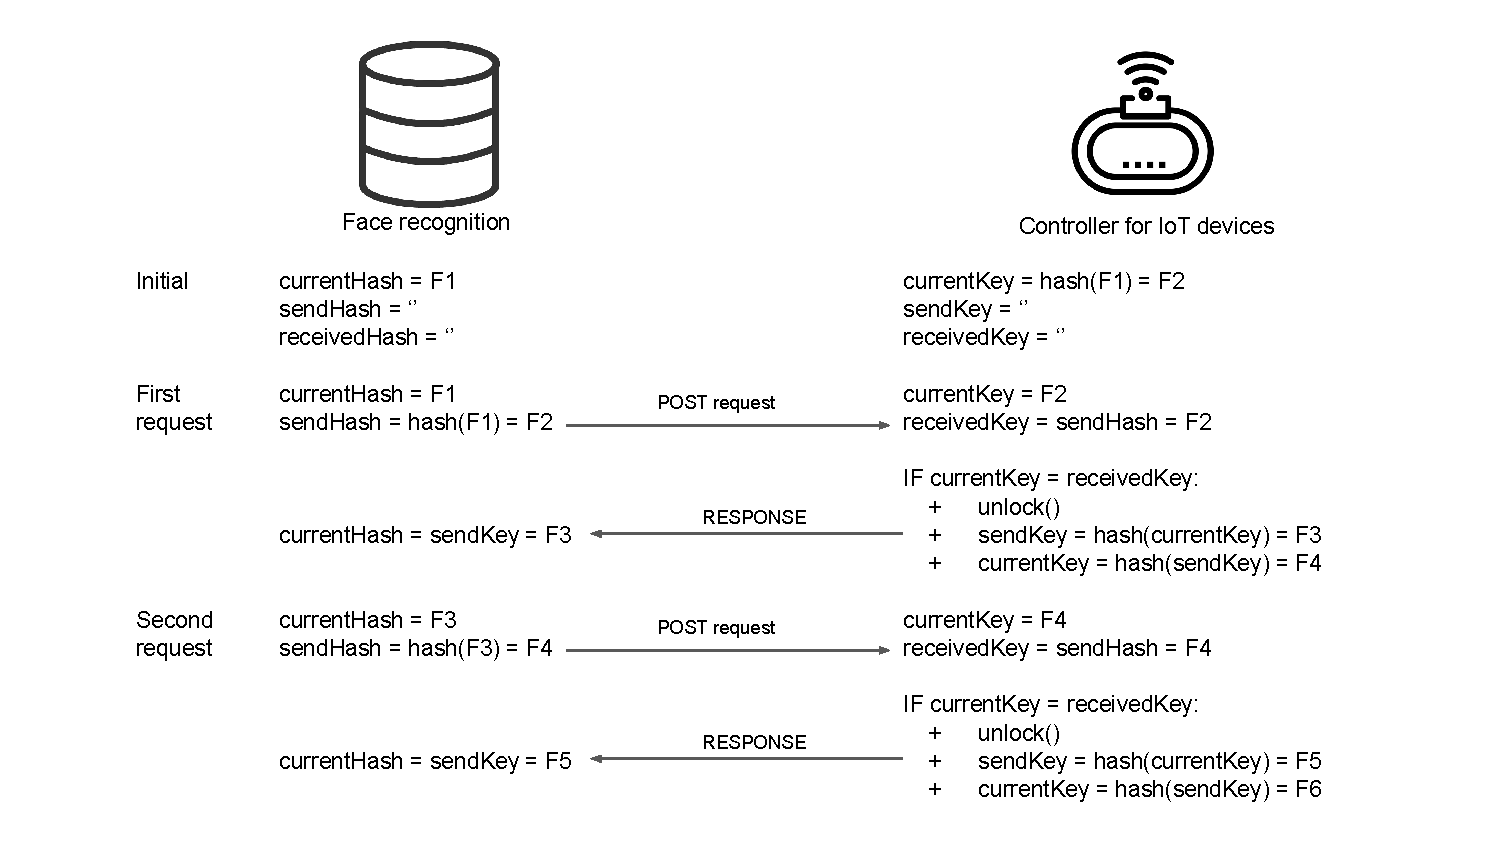
\includegraphics[scale=0.7]{apiDiagram.pdf}
    \caption{API connection flow}
    \label{fig:apiDiag}
\end{figure}

We are applying a blockchain-like method on \acrshort{api} for security. Both server and \acrshort{ccu} has two different initial private key. For example, the initial private key on the server is F1, so the initial of \acrshort{ccu} is SHA-256 encode of F1. After every request, a private key that store on both side change, as shown in figure~\ref{fig:apiDiag}. If someone can hack to the connection, they neither can trace back to the first private key nor find out the encoding algorithm.

Latency in this system is also a problem to be a suitable replacement in real life since they share the same local network, the system work in almost real-time.



% ----------------------- CHAPITRE ---------------------------

\chapter{Result and Discussion}
\label{Result and Discussion}
\section{Experimental scenarios}
Our evaluation is performed on a MacBook Pro as the Face recognition system; Raspberry Pi version 4 as the \acrlong{ccu} to control IoT devices. Table~\ref{tab:serverSpecs} summarizes the hardware configuration. The \acrlong{ccu} hardware configuration is mentioned in table~\ref{tab:raspiSpecsr}.

\begin{table}[H]
    \centering
    \caption{Face recognition server configuration}
    ~\\
    \begin{tabular}{|c|c|}
        \hline
        OS & macOS Mojave 10.14 \\
        \hline
        CPU & Intel(R) Core(TM) i7-3720QM \\
        \hline
        RAM & 16GB\\
        \hline
        GPU & NVIDIA GeForce GT 650M (1GB VRAM)\\
        \hline
    \end{tabular}
    \label{tab:serverSpecs}
\end{table}

\begin{table}[H]
    \centering
    \caption{\acrlong{ccu} specification}
    \begin{tabular}{|c|c|}
        \hline
        OS & Raspberry Pi OS (Linux based) \\
        \hline
        Kernel version & 5.10\\
        \hline
        CPU & Quad-core Cortex-A72 (ARM v8) 64-bit Soc \\
        \hline
        RAM & 4GB\\
        \hline
    \end{tabular}
    \label{tab:raspiSpecsr}
\end{table}

As face recognizing is memory intensive, Raspberry Pi can not compute as fast as on a server. So that to have a better user experience, we are choosing to implement the model on a MacBook Pro for testing. On a retail product, we may have to build up a server for each client.

Figure \ref{fig:prodSetup} shows the device setup diagram for evaluating, testing, and also in the public product:

\begin{figure}[H]
    \centering
    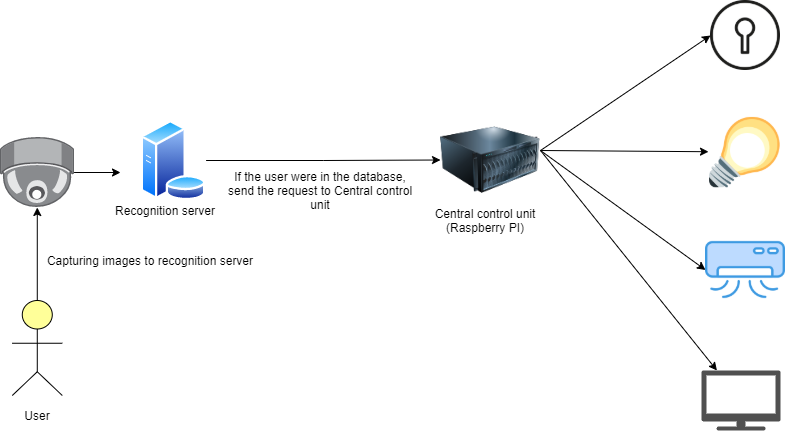
\includegraphics[scale=0.6]{setupDiag.png}
    \caption{Product flow}
    \label{fig:prodSetup}
\end{figure}

\section{System evaluation}
\subsection{Recognition system}
We are evaluating the model as the performance of the recognition system. The Confusion matrix is built to evaluate how well the model is.

\begin{table}[H]
    \centering
    \caption{Confusion matrix}
    \begin{tabular}{|c|c|c|}
        \hline
         &  Actual Negative &  Actual Positive\\
        \hline
        Predict Negative & True Negatives (TN) & False Negatives (FN)\\
        \hline
        Predict Positive & False Positive (FP) & True Positive (TP)\\
        \hline
    \end{tabular}
    \label{tab:confusionMatrix}
\end{table}
\begin{itemize}
    \item \textbf{Accuracy}: Accuracy is the value that shows how accurate  the model is, overall the class.
    \[
        Accuracy = \frac{TN+TP}{TN+FN+TP+FP}
    \]
    \item \textbf{Precision}: Precision defines how good the model is when predicting a class if the precision is low, meaning your model makes many mistakes in predicting.
    \[
        Precision = \frac{TP}{TP+FP}
    \]
    \item \textbf{Recall}: Recall(or Sensitivity) shows the accuracy of your model on the positive case, so the higher Recall, the better your model.
    \[
        Recall = \frac{TP}{TP+FN}
    \]
    \item \textbf{F1 score}: F1 score show the balance between Precision and Recall
    \[
        F1 = 2\times\frac{Precision*Recall}{Precision+Recall}
    \]
\end{itemize}

\begin{table}[H]
    \centering
    \caption{Evaluation with confusion matrix}
    \begin{tabular}{|c|c|c|c|c|}
        \hline
        Accuracy & Precision & Recall & F1 score \\
        \hline
        0.983740 & 0.986542 & 0.982919 & 0.983147 \\
        \hline
    \end{tabular}
\end{table}

We test the effective of the model by using a set of test images that includes many classes. Then the model will extract the embedding vectors for each image. After getting vectors, we use t-sine for reducing the dimensional of the vectors then visualize it.

\begin{figure}[H]
    \centering
    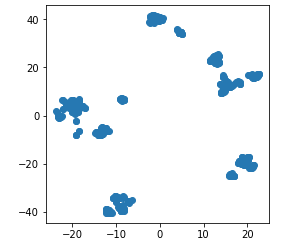
\includegraphics[scale=0.9]{tsneVisual.png}
    \caption{Scatter plot of the embedding vectors}
\end{figure}

For a better visual, we will show it on TensorBoard. The model works flawlessly on moving the picture of a same person together.

\begin{figure}[H]
    \centering
    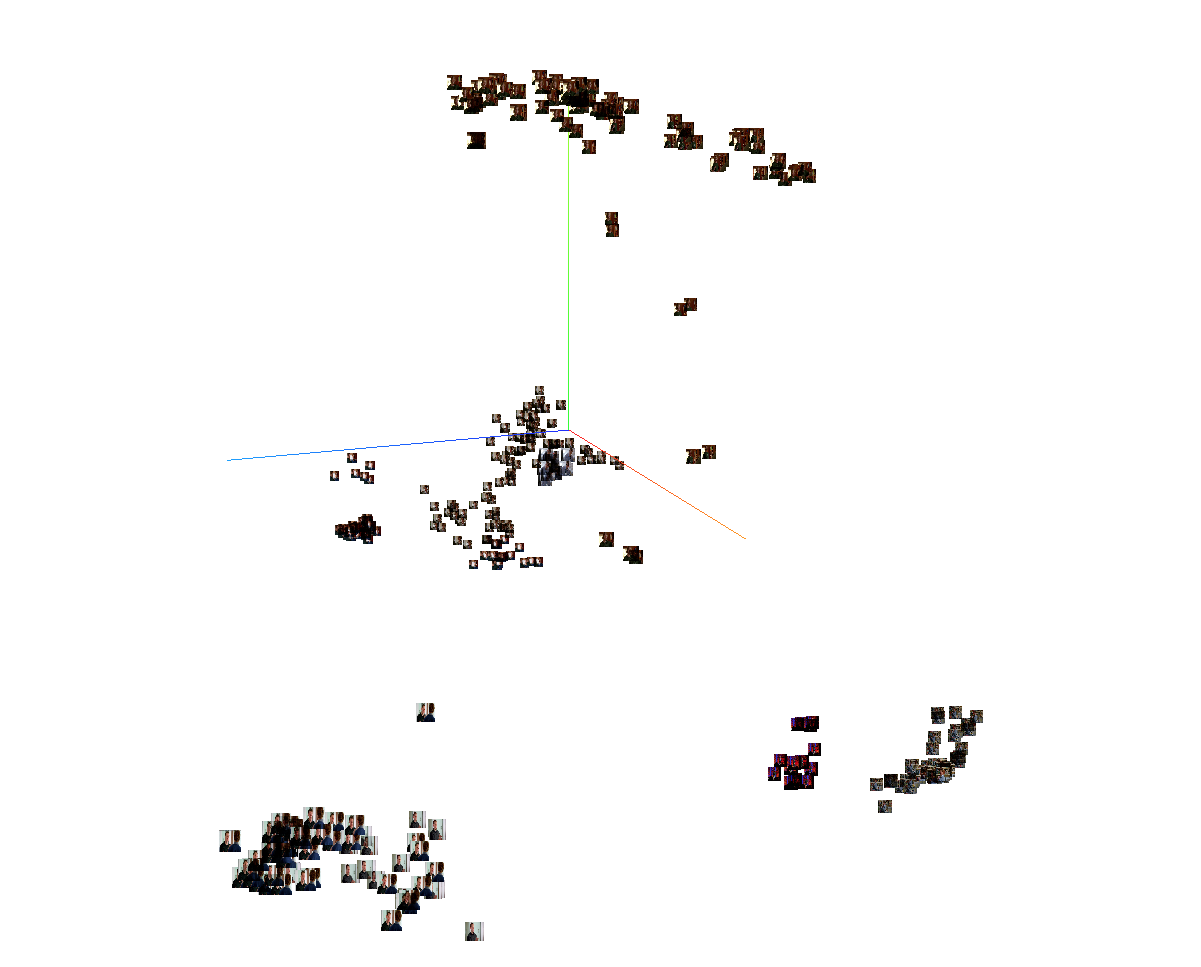
\includegraphics[scale=0.4]{tensorBoard.png}
    \caption{TensorBoard visualisation of embedding vectors}
\end{figure}

We applied the system onto our home on real-time usage, and it has an estimated 95\% accuracy based on successful unlock, failed to unlock.

Table~\ref{tab:trainingTime} shows the time of processing for each scenario (we choose one picture for each class):
\begin{table}[H]
    \centering
    \caption{Processing time for each scenario}
    \begin{tabular}{|c|c|}
        \hline
        Number of the registered person & Processing time(seconds) \\
        \hline
        3 & 2.17\\
        \hline
        100 & 39.18\\
        \hline
        4000 & 313\\
        \hline
    \end{tabular}
    \label{tab:trainingTime}
\end{table}

The processing time above indicates the time of calculating pictures to 128 dimension vectors. It can improve by using better hardware for less executing time.

\subsection{\acrlong{ccu} and \acrshort{api} performance}
\paragraph{}
The performance of \acrshort{ccu} is calculated on the percentage of success time and failed time. For most of the testing time, the system runs perfectly with a 100\% success rate.

About the \acrshort{api} connection, the only network connection can affect its performance. Since we shared a local network on both devices, \acrshort{api} runs without any delay.

\section{Discussion}
In everyday usage, our system works without any problems. But compare with other products on the market, there are some drawbacks to our approach:
\subsubsection{Inaccuracy with an extensive database}
\paragraph{}
On our evaluation, with an extensive database (more than 4000 people), the model seems not to recognize as accurately as before. Many elements can affect the performance, but we think that in a sizeable registered person, there will be a small percentage that two people can have a similar face landmarks as well as similar Euclidean vectors. That leads to an equal distance when compare them to each other.

We think that our model is not trained enough to extract more precise face landmarks. This problem can be solved by a well-trained model with a large dataset.

\subsubsection{Set up the system on multiple devices}
\paragraph{}
Many public products by large company that integrated all elements on only one device like in ~\ref{fig:publishedProd}. Compare with our product in ~\ref{fig:ccuSetup}, we have to implement it on two devices: one for recognition and one for control the lock, as well as other smart home devices.

\begin{figure}[H]
    \centering
    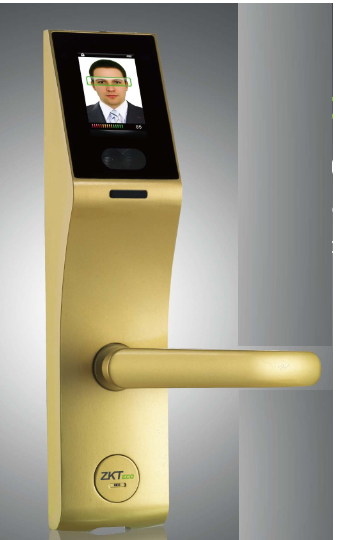
\includegraphics[scale=0.6]{marketProduct.png}
    \caption{An example of an on-sale product}
    \label{fig:publishedProd}
\end{figure}

\begin{figure}
    \centering
    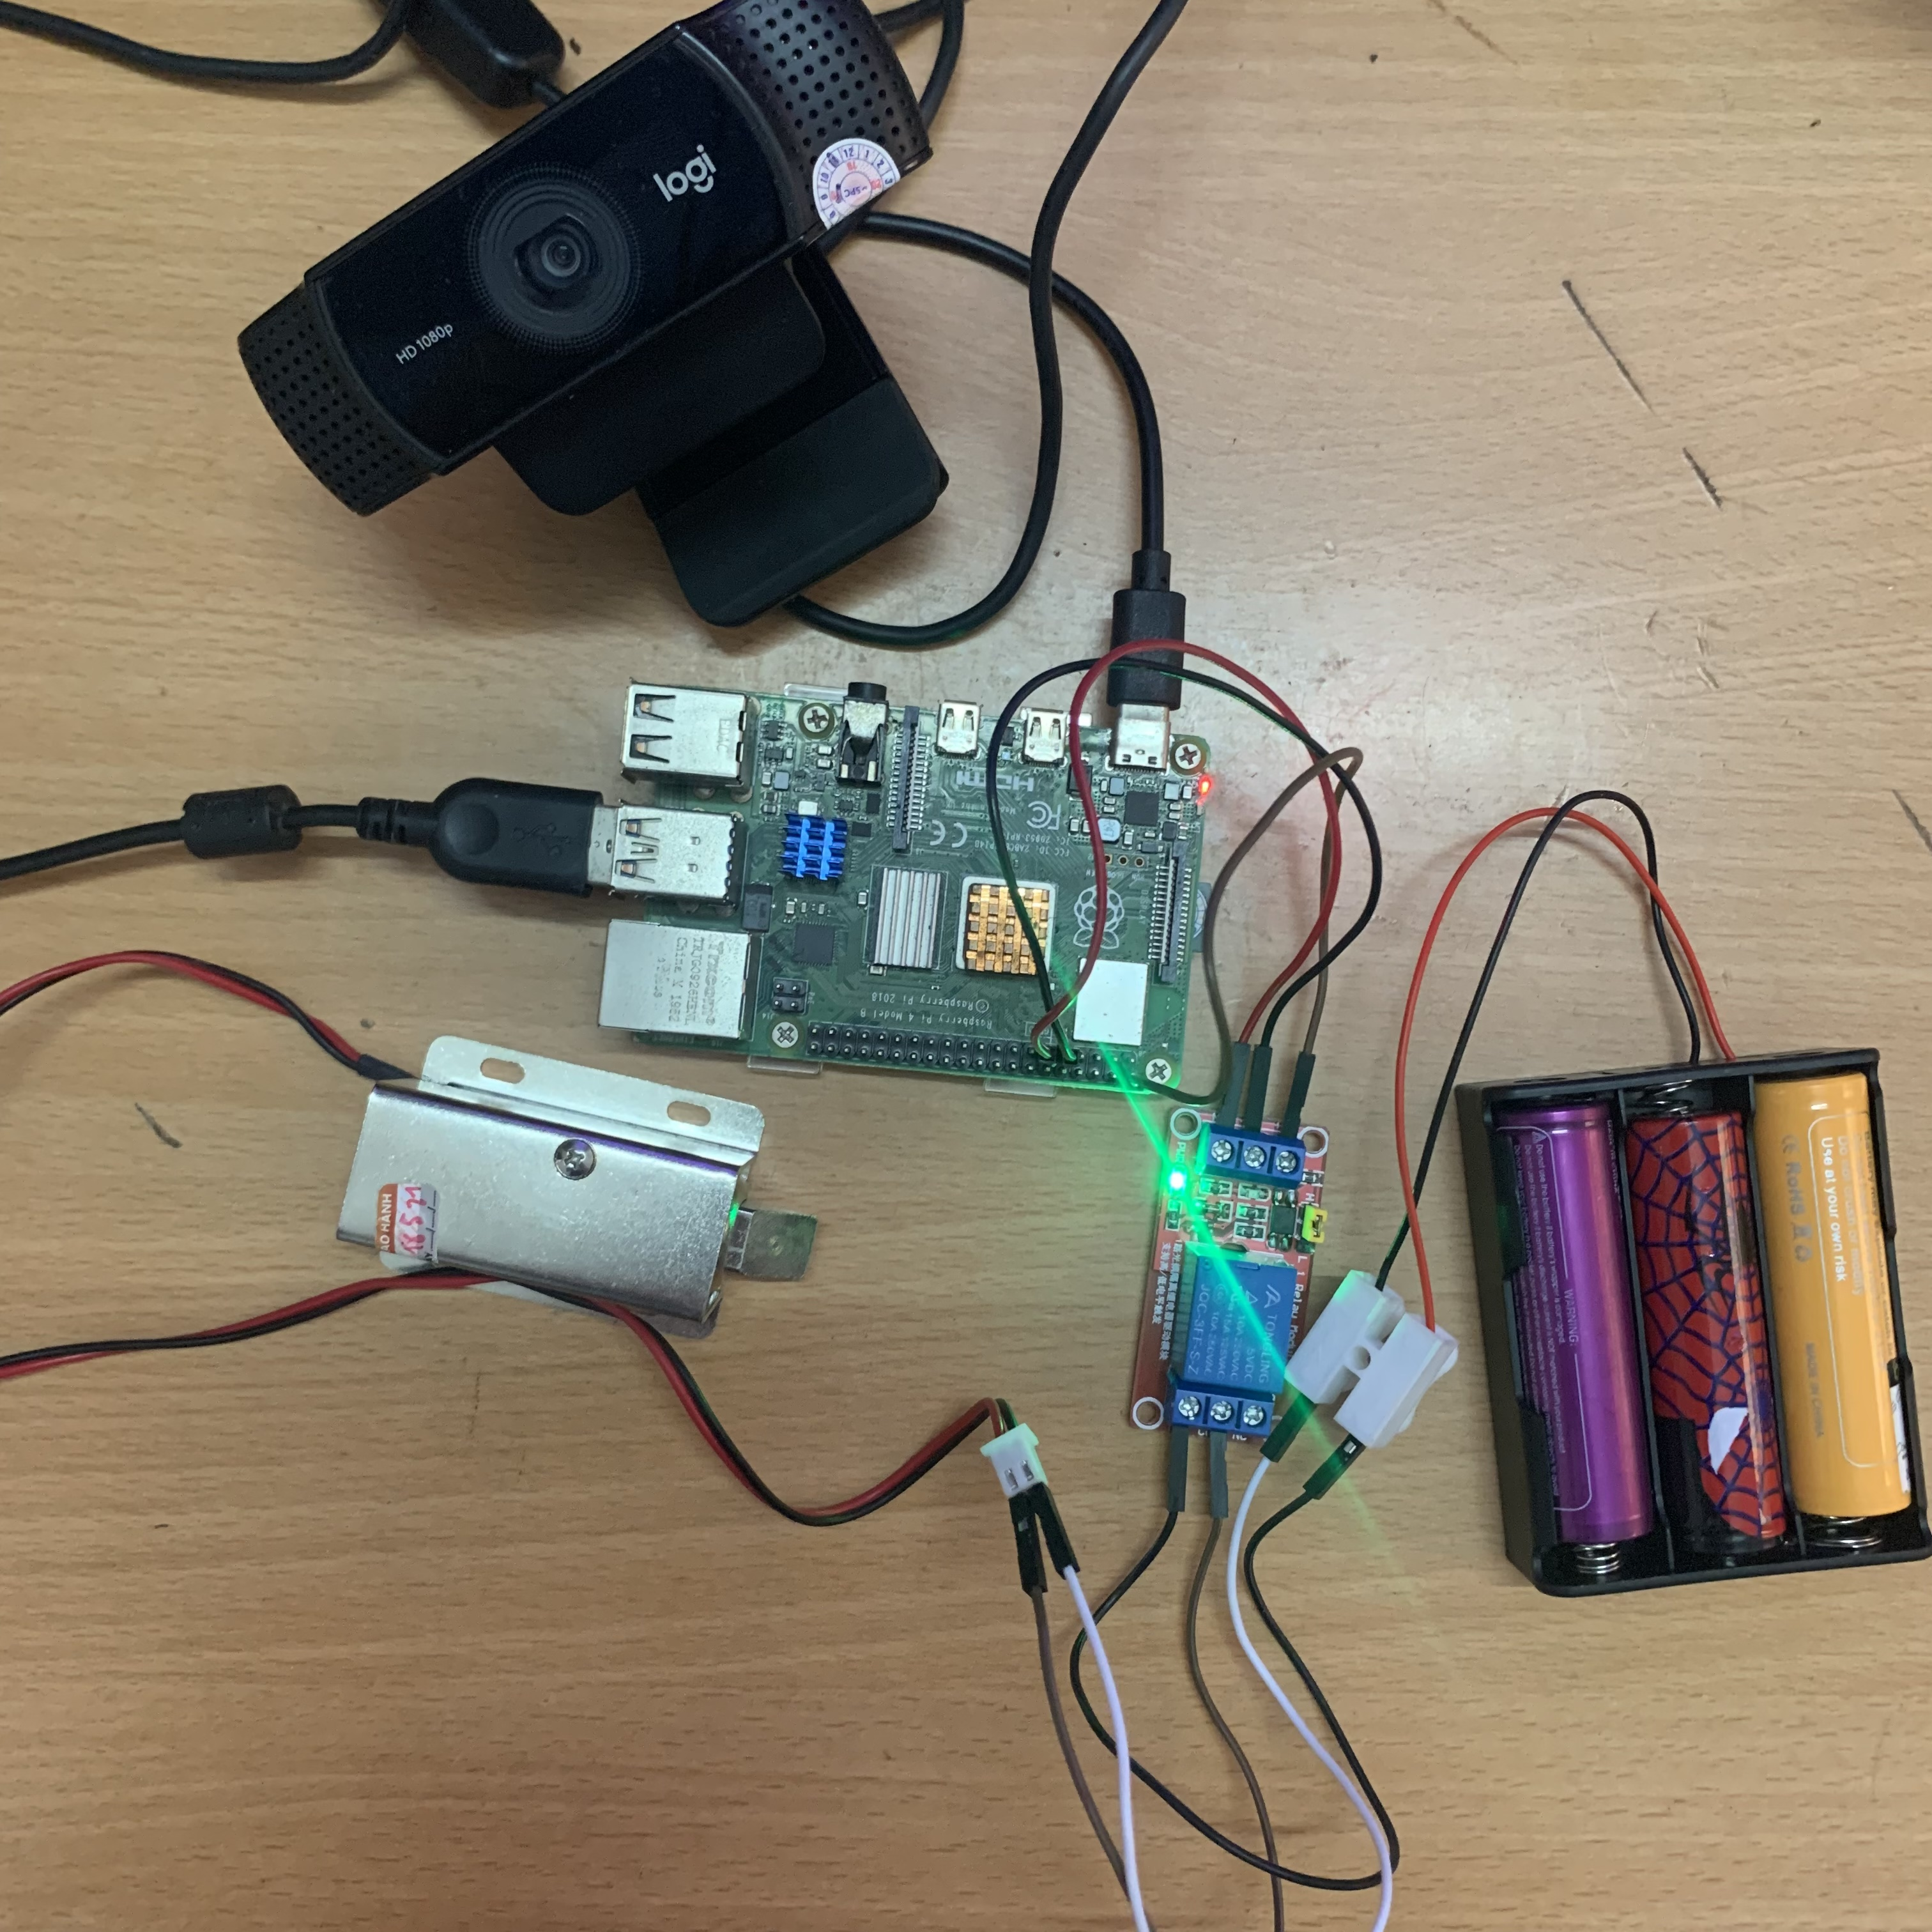
\includegraphics[scale=0.16]{ccuSetup.jpeg}
    \caption{Our door lock setup}
    \label{fig:ccuSetup}
\end{figure}

We have tried to implement the recognition system on the \acrshort{ccu}. Still, since it was relatively computationally and memory intensive, the recognition has the worst performance when running on the \acrshort{ccu}.




% ----------------------- CHAPITRE ---------------------------

\chapter{Conclusion and Future-work}
\paragraph{}
Face recognition is a new security solution. Despite that many companies still prefer traditional ways for security like door locks using keys or fingerprint locks, face recognition still shows its strength in the easy to use and fast for customers. Looking to a post-\acrshort{covid-19} world, we believe that the investment in a facial recognition system now will be cost-effective in the long run.\par


Three months of internship is precious for understanding many concepts of machine learning. Besides the work I have done, I have been thinking of improving the model and expanding the system. Rather than using only one photo for each class, we can apply Data Augmentation to broaden the training dataset but not making the user inconvenient in taking many photos. And I am thinking of creating a model smaller that can fit a mobile app. That way can expand the usage of this work to many devices. 

% ----------------------- BIBLIOGRAPHIE ---------------------------
\addcontentsline{toc}{chapter}{Bibliography}
\bibliography{Biblio}
\bibliographystyle{unsrt}

% ----------------------- ANNEXES ---------------------------

\appendix
\include{Appendix}




\end{document}
